\documentclass[11pt]{article}
\usepackage{amsmath}
\usepackage{graphicx}
\usepackage{caption}
\usepackage{amssymb}
\usepackage{verbatim}
\usepackage{hyperref}
\usepackage{listings}
\usepackage{float}
\usepackage[thinc]{esdiff}
\usepackage{euscript}
\usepackage{subcaption}
\usepackage{commath}
\setlength{\parindent}{0em}
\newcommand*{\field}[1]{\mathbb{#1}}%
\usepackage{amsthm}
\newtheorem{claim}{Claim}
\captionsetup{labelformat=empty}

\begin{document}
\begin{titlepage} % Suppresses displaying the page number on the title page and the subsequent page counts as page 1
	
	\center % Centre everything on the page
	
	\vspace*{3cm}

	\textsc{Mathematical Tripos, Part 1B}\\
	\textsc{Computational project}
	\begin{center}
      {\huge\bfseries The Restricted Three-Body Problem\\[0.4cm]
}     \end{center}
	 % Title of your document
	
	\vfill
	\vfill\vfill
	
	\includegraphics*[width = 2.675cm, height = 3.1cm]{coat.png}
	\vfill
	\textsc{University of Cambridge}
	%------------------------------------------------
	%	Date
	%------------------------------------------------
	\vspace*{\fill}
	\vfill\vfill
	{\large\today} 
	\vfill
	% Push the date up 1/4 of the remaining page	
\end{titlepage}
\section{Introduction}
\subsection{Question 1}
From project introduction, we have the following equations:
\begin{align*}
\ddot{x} - 2\dot{y} &= -\frac{\partial \Omega}{\partial x}    
&\tag{1.1a}\\
\ddot{y} - 2\dot{x} &= -\frac{\partial \Omega}{\partial y}
  &\tag{1.1b}
\end{align*}
And
\begin{equation*}
\Omega = -\frac{1}{2}(x^{2}+y^{2})-\frac{\mu}{\sqrt{(x+1-\mu)^{2}+y^{2}}}-\frac{1-\mu}{\sqrt{{(x-\mu)}^{2}+y^{2}}} \tag{1.2}
\end{equation*}
Which has time derivative:
$$\dot{\Omega} = \frac{\partial \Omega}{\partial x} \dot{x}+\frac{\partial \Omega}{\partial y} \dot{y} = (2\dot{y}-\ddot{x})\dot{x}+(2\dot{x}-\ddot{y})\dot{y}= -(\dot{x} \ddot{x}+\dot{y} \ddot{y}) $$
The quantity $$ \mathit{J} = \frac{1}{2}({\dot{x}}^{2}+{\dot{y}}^{2})+\Omega(x,y)$$ has time derivative:
$$\dot{\mathit{J}} = \dot{x}\ddot{x}+\dot{y}\ddot{y}+\dot{\Omega} = 0$$
Therefore it is a constant of the motion.
Hence, $$\frac{1}{2}({\dot{x}}^{2}+{\dot{y}}^{2})+\Omega(x,y) = \mathit{J}(x, y) = \mathit{J}(x_{0},y_{0}) = \Omega(x_{0},y_{0})+\frac{1}{2}(u_{0}^{2}+v_{0}^{2}) $$
Therefore, we have the following
$$\Omega(x,y) = \Omega(x_{0},y_{0})+\frac{1}{2}(u_{0}^{2}+v_{0}^{2})-\frac{1}{2}({{\dot{x}}^{2}+{\dot{y}^{2}}})\leqslant\Omega(x_{0},y_{0})+\frac{1}{2}(u_{0}^{2}+v_{0}^{2})$$
equality holds when $\dot{x} = \dot{y} = 0$
\subsection*{Programming Task} See appendix
\section{Space travel}
\subsection{Question 2}
Given that the spaceship is close enough to $P_{h}$, (2) becomes
\begin{equation*}
\Omega = -\frac{0.5}{\sqrt{(x-\mu)^{2}+y^{2}}} 
\end{equation*}
Apply coordinate transformation $x(t)-\mu = r(t)\cos\theta(t),\ y(t) = r(t)\sin\theta(t)$, we obtain:
\begin{align*}
\dot{x} &= \dot{r} \cos \theta-r \sin \theta \dot{\theta} 
\\
\dot{y} &= \dot{r} \sin \theta+r \cos \theta \dot{\theta}
\\
\ddot{x} &= \ddot{r}\cos\theta -2\dot{r} \sin\theta \dot{\theta} -r\cos\theta {\dot{\theta}}^{2}-r\sin\theta\ddot{\theta}
\\
\ddot{y} &= \ddot{r}\sin\theta + 2\dot{r}\cos\theta\dot{\theta}-r\sin\theta\dot{\theta}^2+r\cos{\theta}\ddot{\theta}
\\
\end{align*}
And 
\begin{align*}
\frac{\partial \Omega}{\partial x} &= \frac{\cos\theta}{2r^{2}} \\
\frac{\partial \Omega}{\partial y} &= \frac{\sin\theta}{2r^{2}} 
\end{align*}
Hence, after evaluating $\cos\theta*(1a)+\sin\theta*(1b)$ and $\sin\theta*(1a)-\cos\theta*(1b)$,
\begin{align*}
\ddot{r}-r{\dot{\theta}}^{2}-2r\dot{\theta} &= -\frac{1}{2r^{2}}
&\tag{2.1.1a}\\
2\dot{r}+r\ddot{\theta}+2\dot{r}\dot{\theta} &= 0
&\tag{2.1.1b}\\
\end{align*}
from (2.1.1b) we have the following:$$\frac{d(r^{2}\dot{\theta})}{dt}= -2r\dot{r} \Longrightarrow r^{2}\dot{\theta} = k-r^{2}
$$ i.e.$$\dot{\theta} = -1+kr^{-2}$$where k is an arbitrary constant.
Then from (2.1.1a) we have: $$\ddot{r} - r(-1+kr^{-2})^{2}-2r(-1+kr^{-2})= -\frac{1}{2r^{2}}$$i.e.
$$\ddot{r} =\frac{k^{2}}{r^{3}}-\frac{1}{2r^{2}}-r=-V'(r)$$
So $$V'(r) = -\frac{k^{2}}{r^{3}}+\frac{1}{2r^{2}}+r \Longrightarrow V(r) = \frac{k^{2}}{2r^{2}}-\frac{1}{2r}+\frac{r^{2}}{2}+C$$
where C is an arbitrary constant.
If the spaceship moves in a circular orbit with radius a, then we have the following constraint $r = a$, and then $\dot{r} = \ddot{r} = 0$.
\newline 
Therefore, from (2.1.1b) we have $\ddot{\theta} = 0,\ \dot{\theta} = const$ and from (2.1.1a) we have $\dot{\theta}^{2}+2\dot{\theta} - \frac{1}{2a^{3}}= 0 $, take the positive root $\omega = -1+\sqrt{1+\frac{1}{2a^{3}}}$.
Then the initial conditions for circular motion are as follow:
$$\dot{r(0)} = 0,\ \dot{\theta(0)} = \omega,\ r(0) = a,\ \theta(0) = 0$$ which corresponds to the initial conditions in Cartesian coordinates:
$$x(0) = \mu+a,\ y(0) = 0,\ \dot{x(0)} = 0,\ \dot{y(0)} = a\omega $$
From $\ddot{r} = 0$, $$-\frac{k^{2}}{a^{3}}+\frac{1}{2a^{2}}+a = 0$$ and since $\omega>0$,
$$k = \sqrt{\frac{a}{2}+a^{4}}$$. 
The analytic periodic solution is: $x = \mu + a\cos(\omega t),\ y = a\sin(\omega t),\ \dot{x} = -a\omega\sin(\omega t),\ \dot{y} = a\omega\cos(\omega t)$.
\newline
Put in the initial values for a = 0.01 and run the solver, I have the following graph:
\begin{figure}[H]
\centering
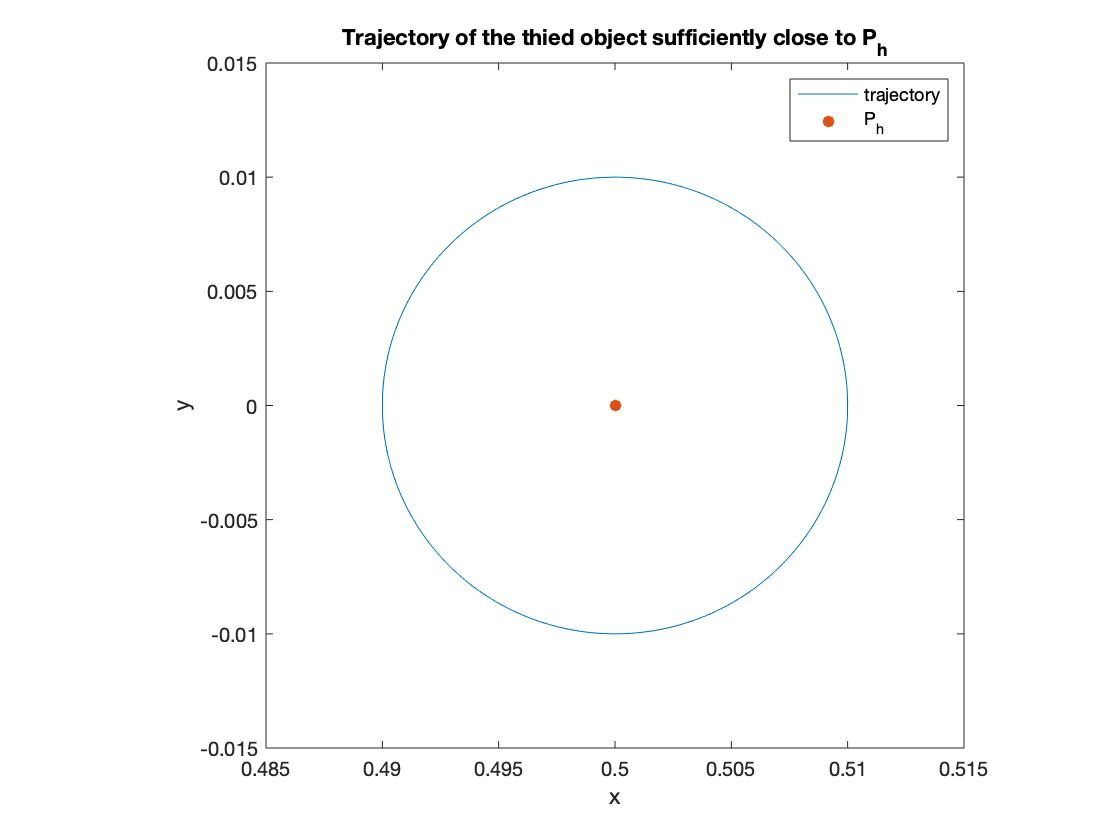
\includegraphics[width = 12cm, height =9cm]{Q2.jpg}
\caption{Figure 2.1: Numerical solution of the system for a = 0.01}
\end{figure}
which is precisely a circular motion.
\subsection{Question 3}
The graphs show the forbidden region (teal) of this motion. 
\newpage
\begin{figure}[H]
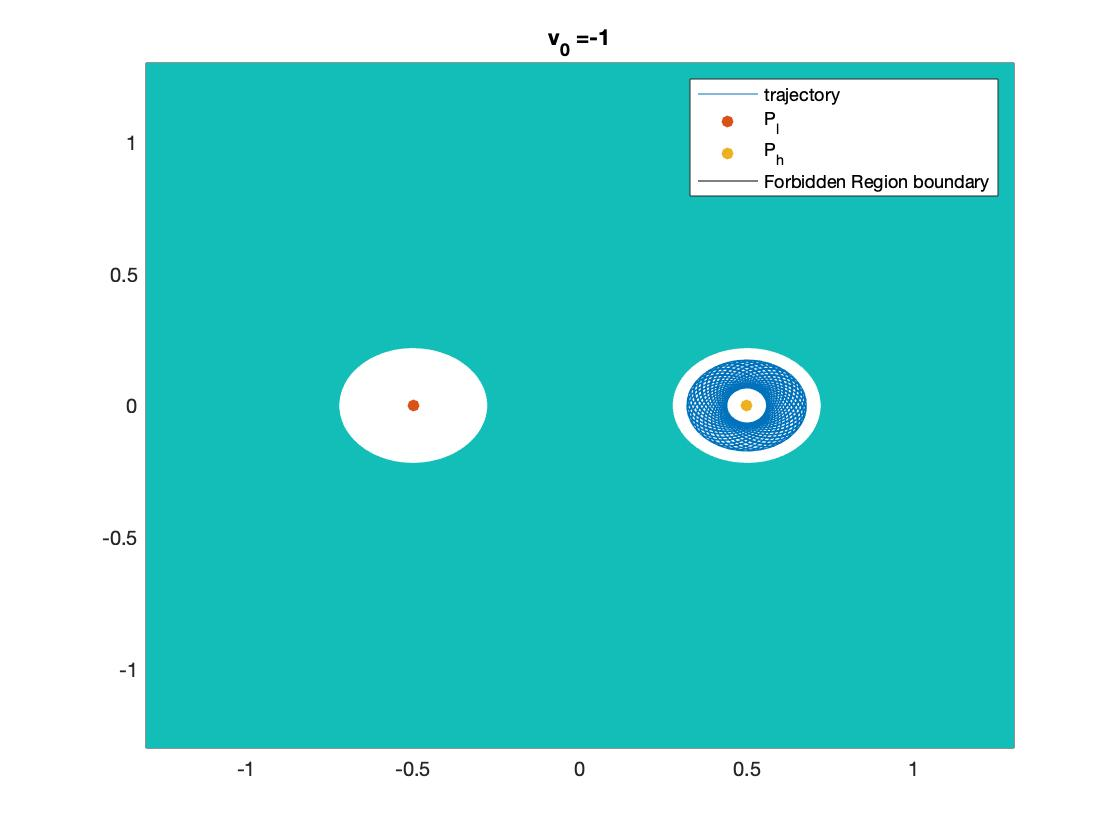
\includegraphics[width = 12cm, height =9cm]{Q3(1).jpg}
\caption{x(30) = 0.4280,  y(30) = -0.0666 }
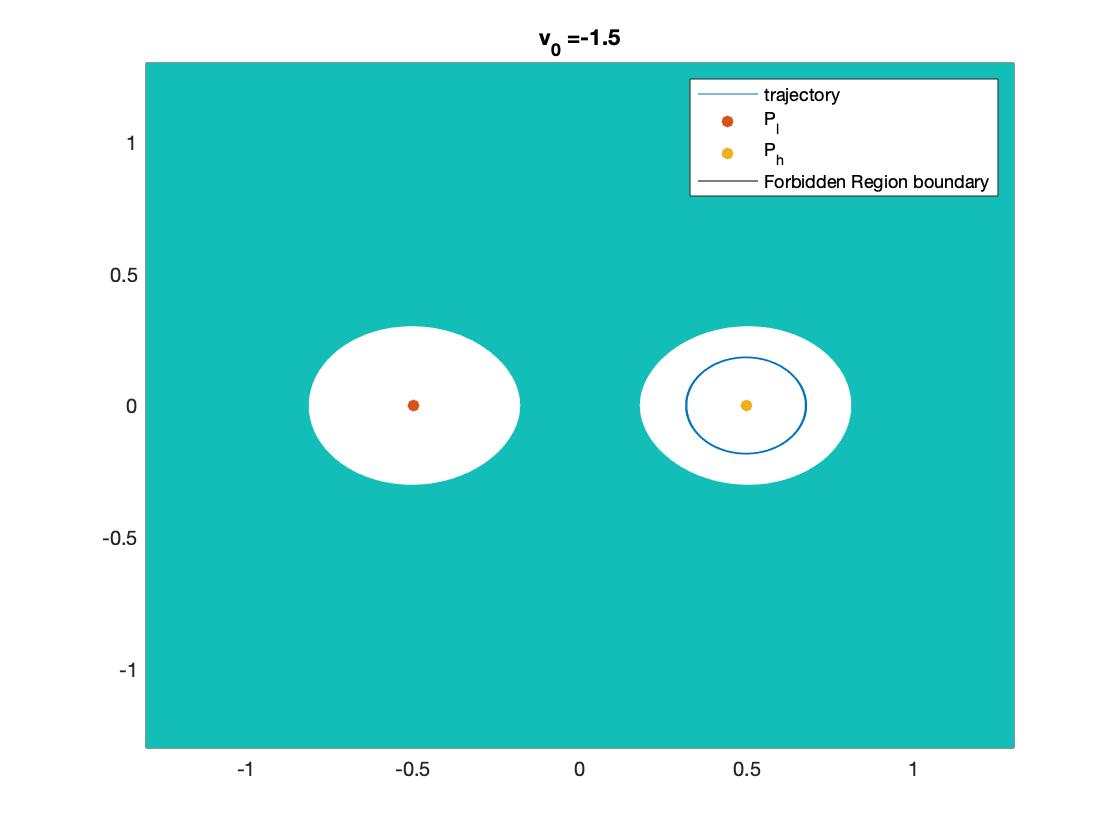
\includegraphics[width = 12cm, height = 9cm]{Q3(2).jpg}
\caption{x(30) = 0.3215,  y(30) = 0.0415}
\end{figure}
\begin{figure}[H]
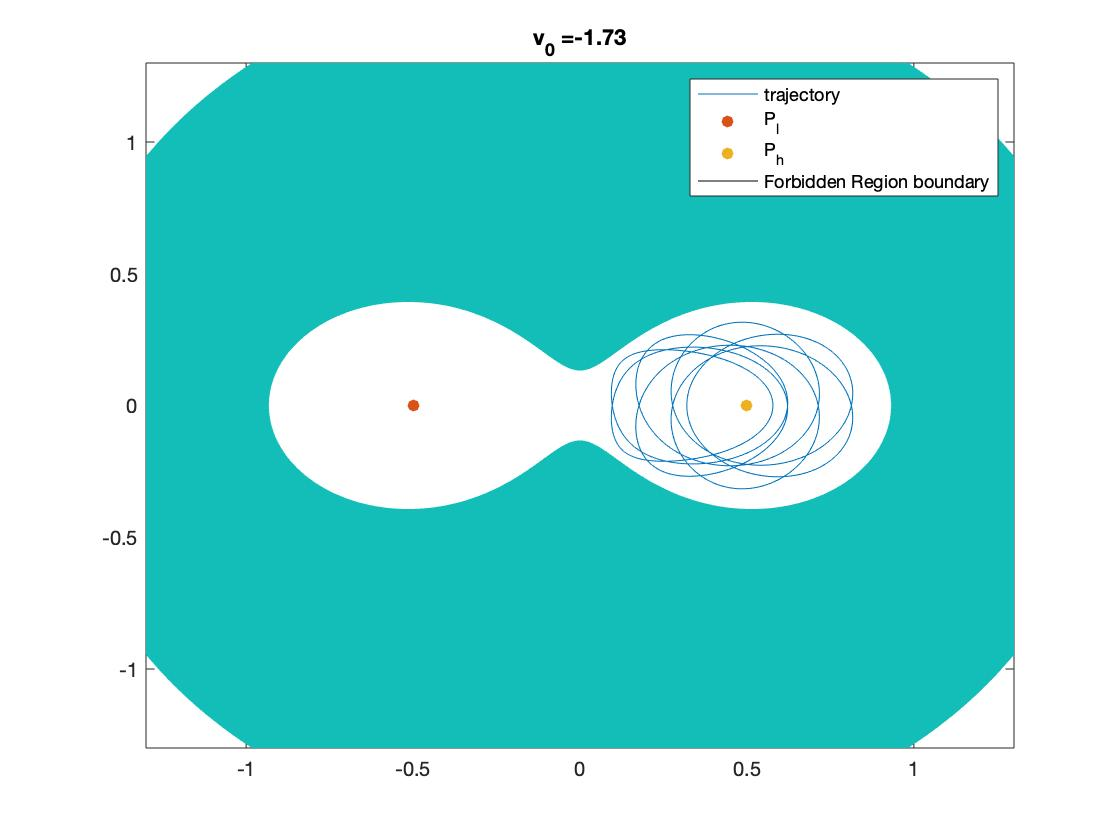
\includegraphics[width = 12cm, height =9cm]{Q3(3).jpg}
\caption{x(30) = 0.1820,  y(30) = 0.1696}
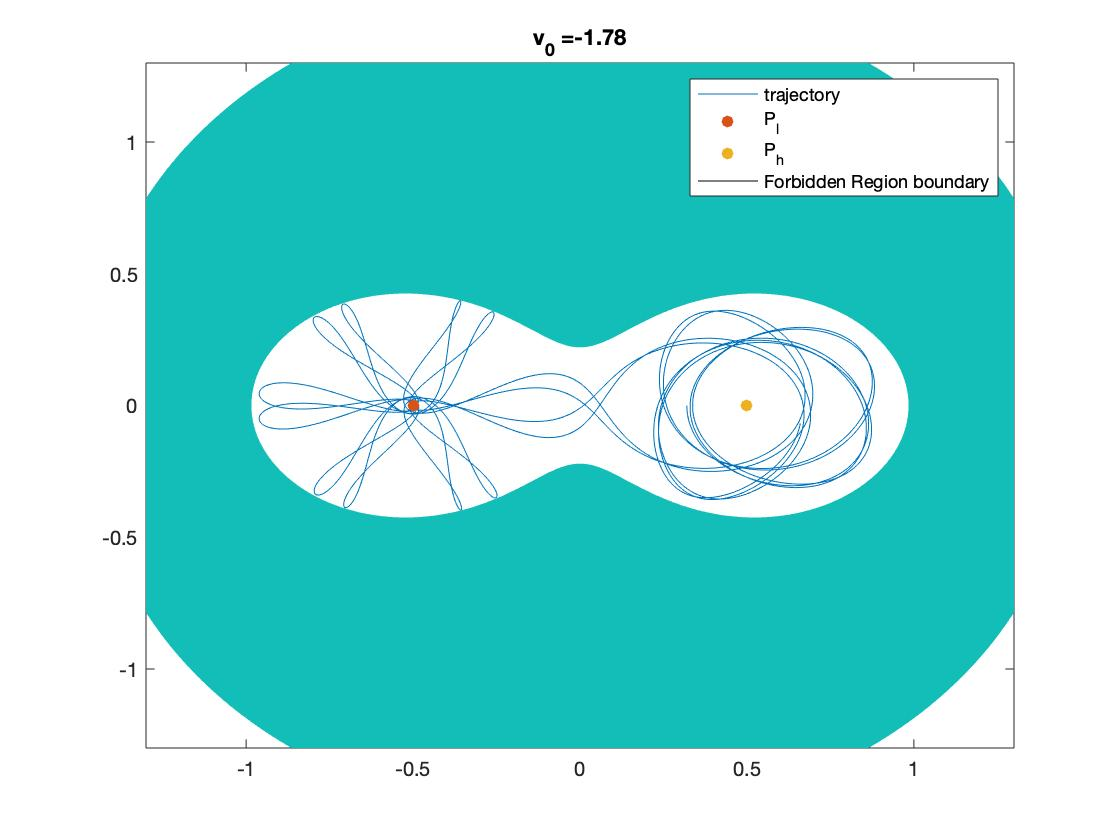
\includegraphics[width = 12cm, height =9cm]{Q3(4).jpg}
\caption{x(30) = 0.6597,  y(30) = -0.0675}
\end{figure}
\begin{figure}[H]
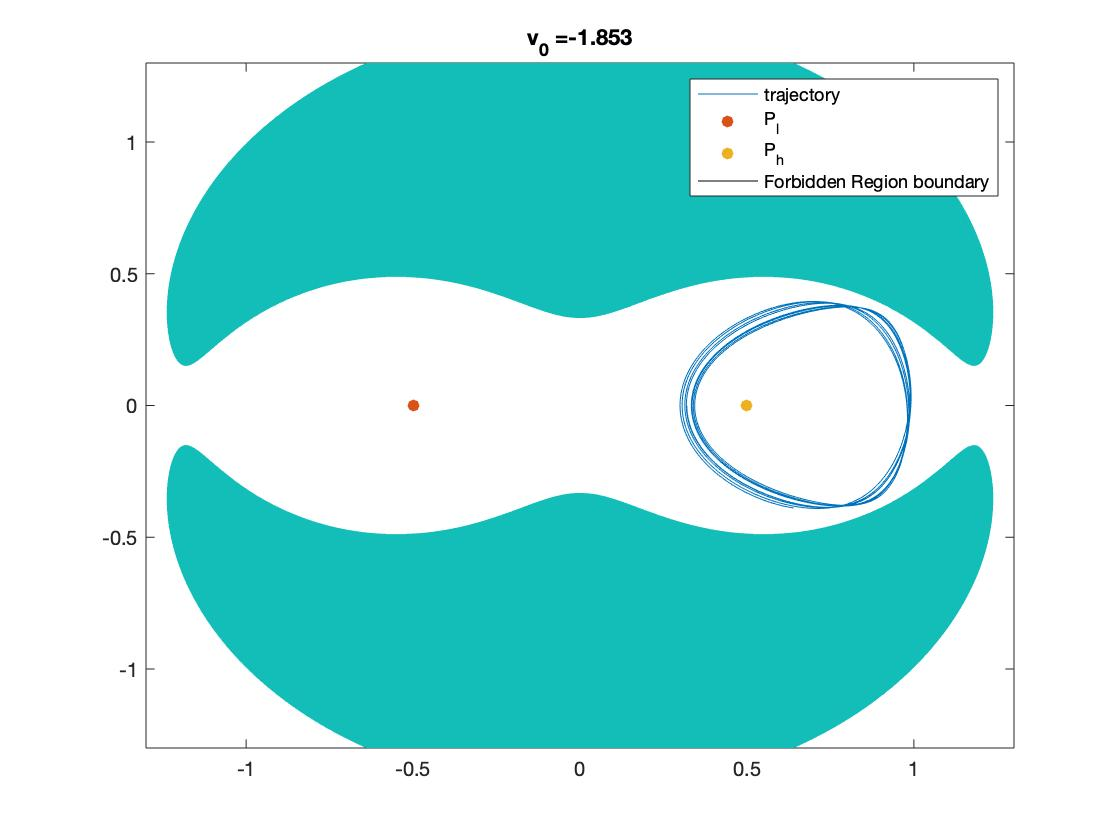
\includegraphics[width = 12cm, height =9cm]{Q3(5).jpg}
\caption{x(30) = 0.6400,  y(30) = -0.3890}
\end{figure}

The relative tolerance accounts for the accuracy of each component of the solution, these graphs are accurate to the tenth significant figure as I have set the relative tolerances to 1e-10. The absolute tolerance is for the solution when it approaches 0, and as the solution for each $v_0$ is at a distance much greater than 1e-10 from 0, they are precise.
The trajectories are elliptical, and as $-v_0$ increases, the eccentricity get larger. The third body gradually overcomes of the potential barrier of $P_h$ and the forbidden region shrunk as the initial constant J increases with $\abs{v_0}$.The allowed the region is a useful guide to the size of the trajectory Therefore when we move from $P_h$ to $P_l$ it would be most suitable to choose $v_0 = -1.78$.
\section{Lagrange points and asteroids}
\subsection{Question 4}
\newpage
\begin{figure}[H]
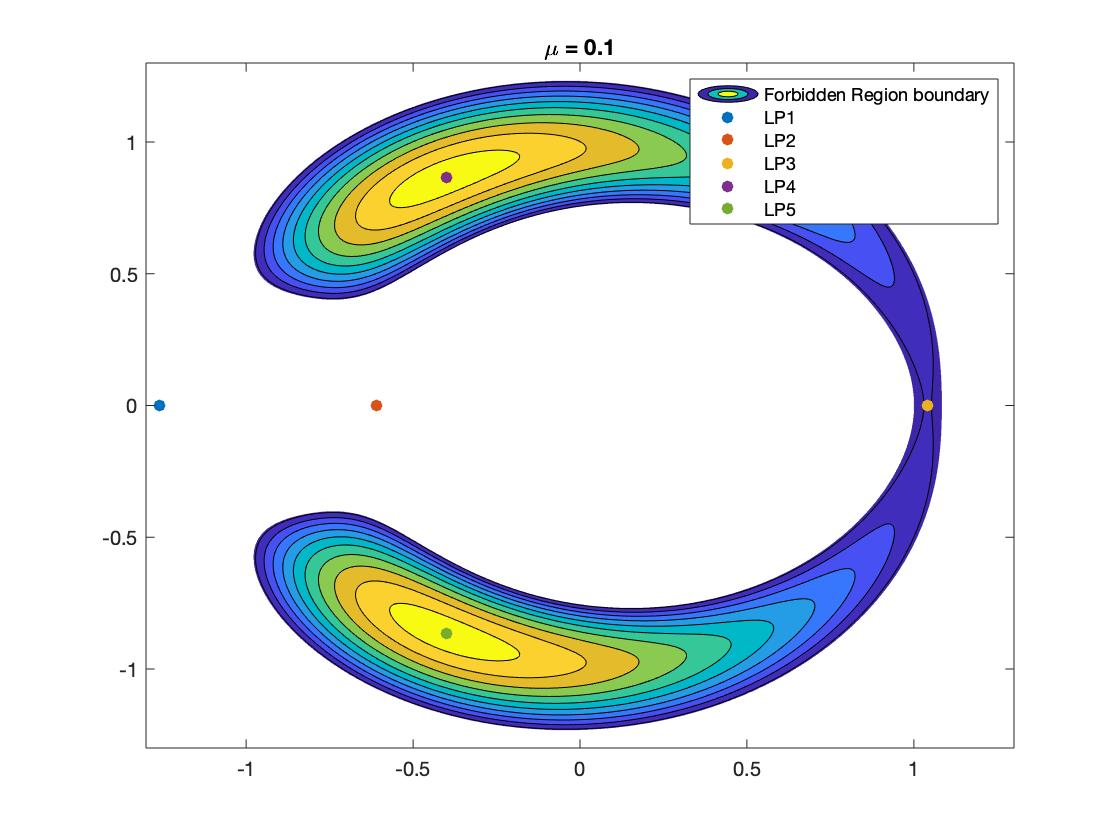
\includegraphics[width = 12cm, height = 8cm]{Q4(1)}
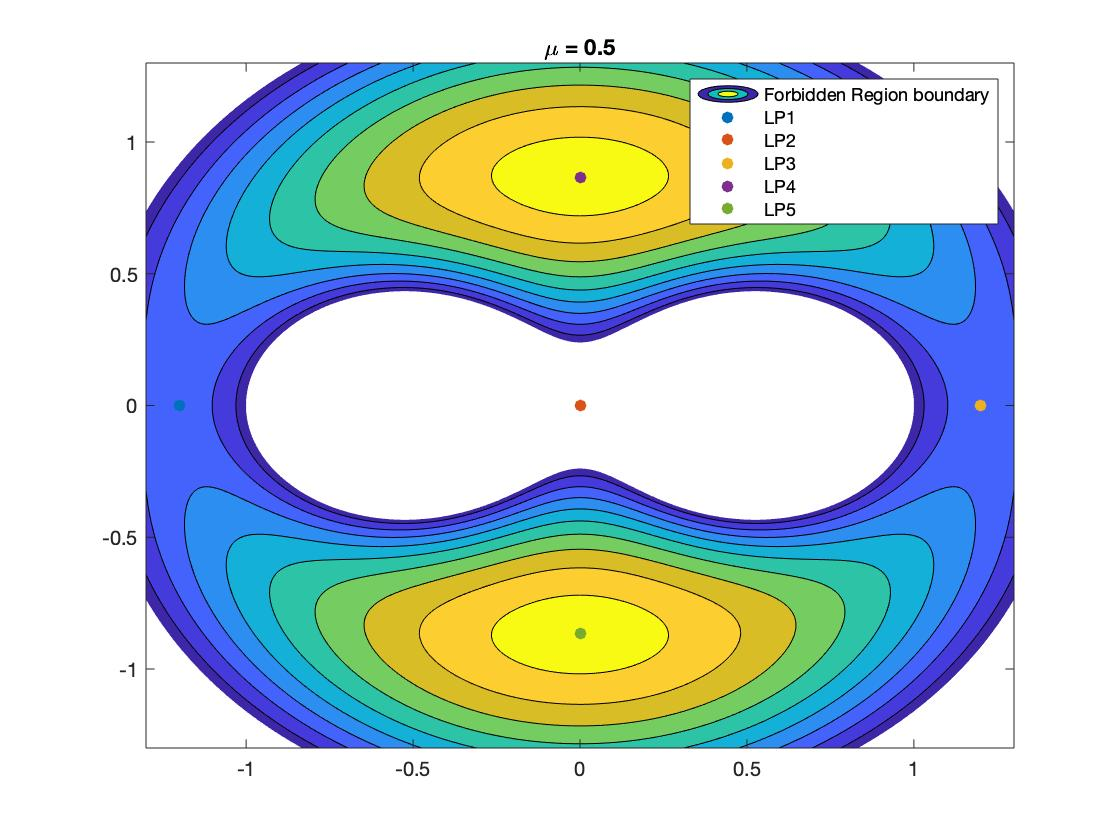
\includegraphics[width = 12cm, height = 8cm]{Q4(2)}
\end{figure}
\begin{figure}[H]
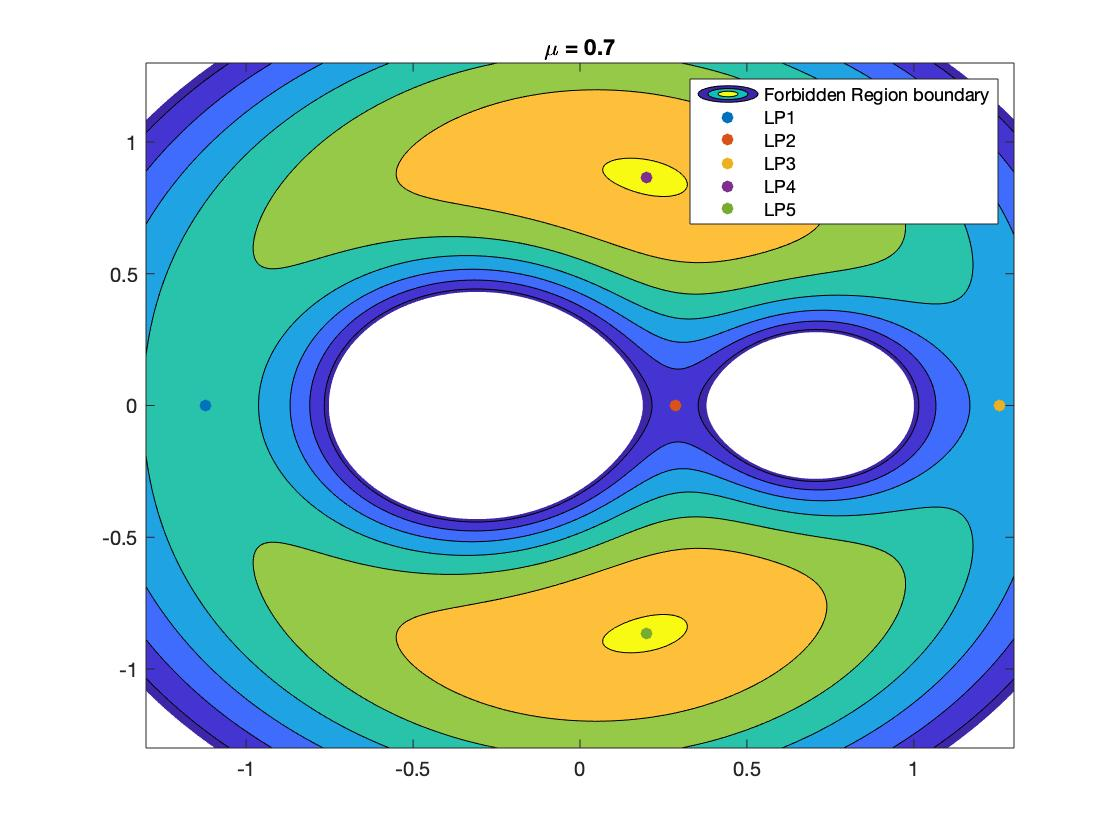
\includegraphics[width = 12cm, height = 8cm]{Q4(3)}
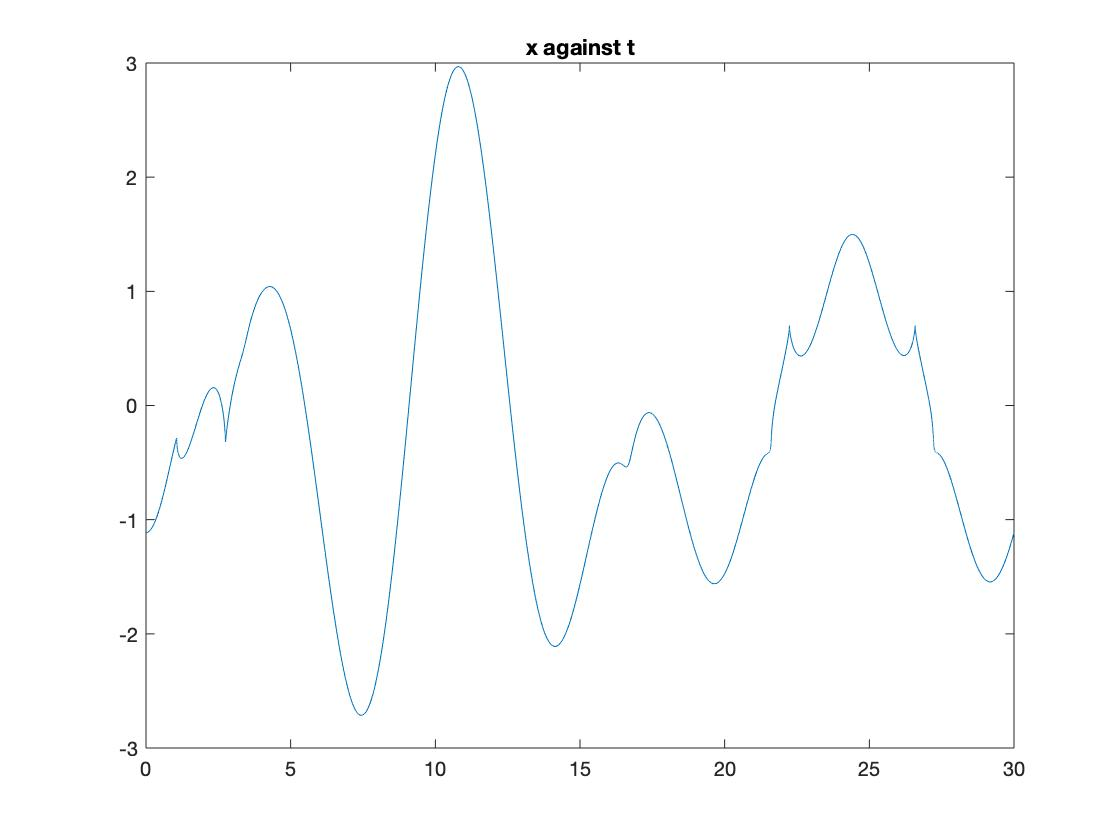
\includegraphics[width = 12cm, height = 8cm]{Q4(4)}
\end{figure}
\begin{figure}[H]
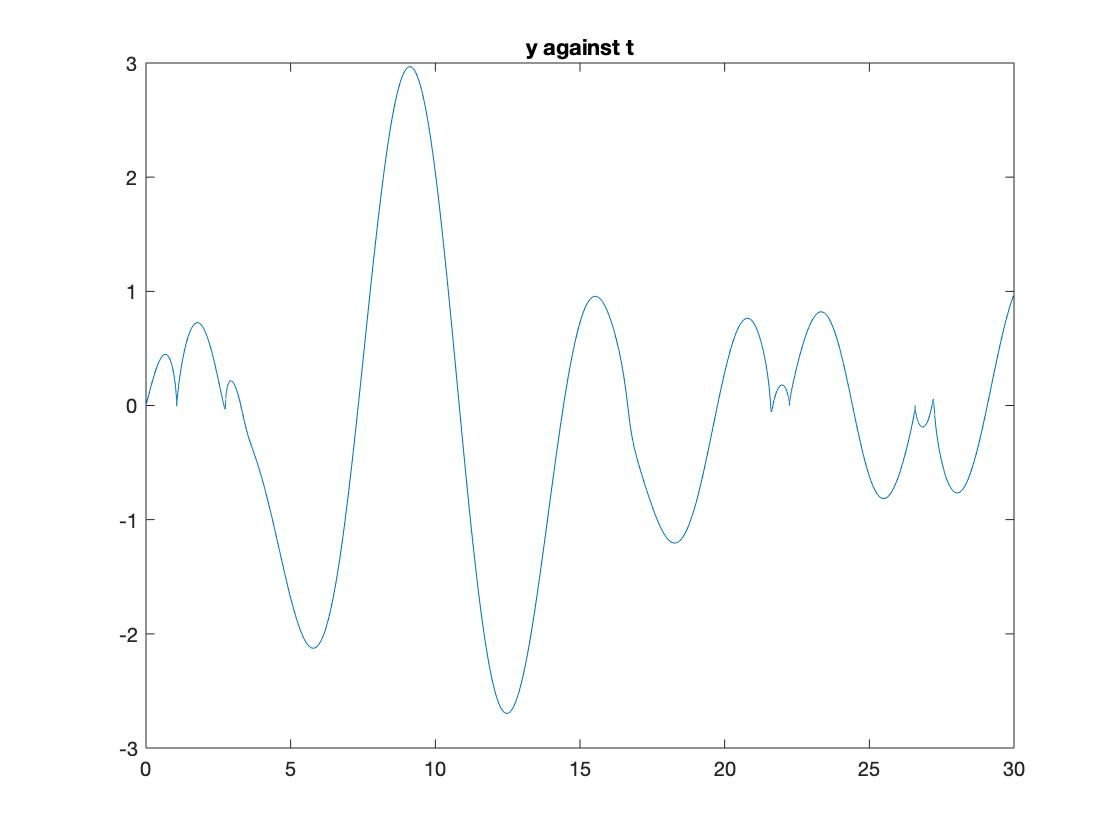
\includegraphics[width = 12cm, height = 8cm]{Q4(5)}
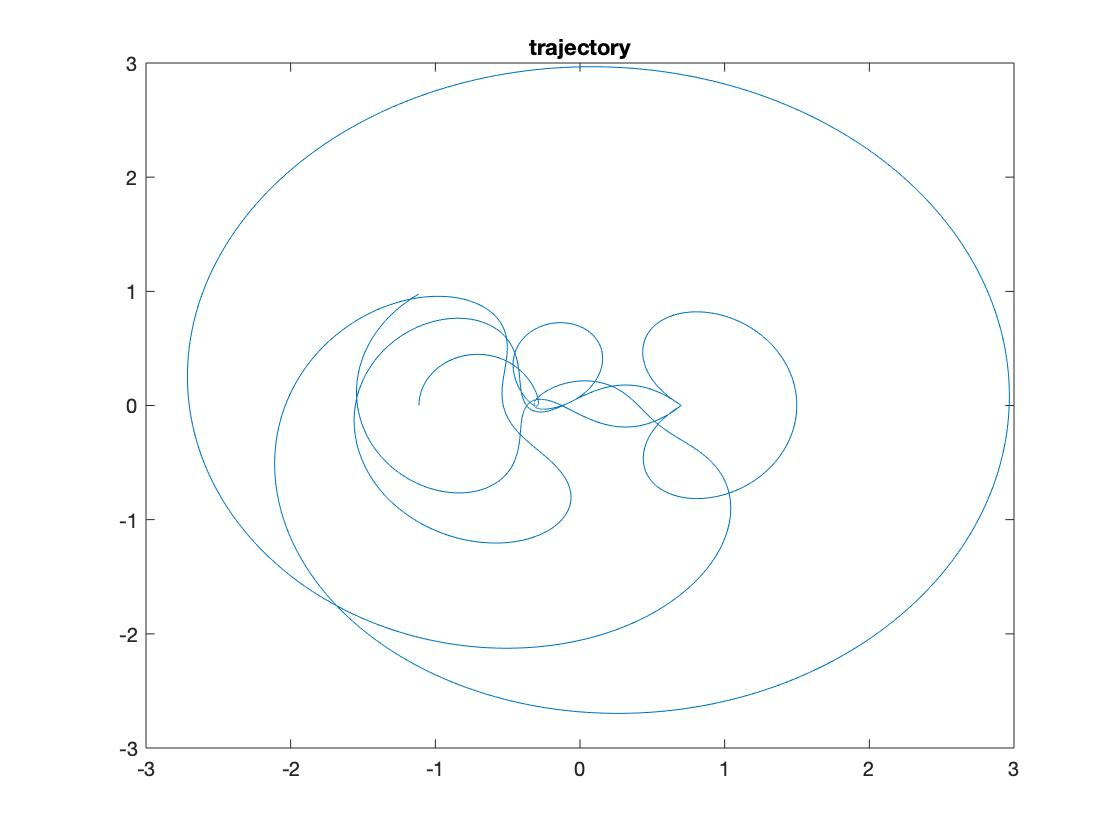
\includegraphics[width = 12cm, height = 8cm]{Q4(6)}
\end{figure}
\begin{figure}[H]
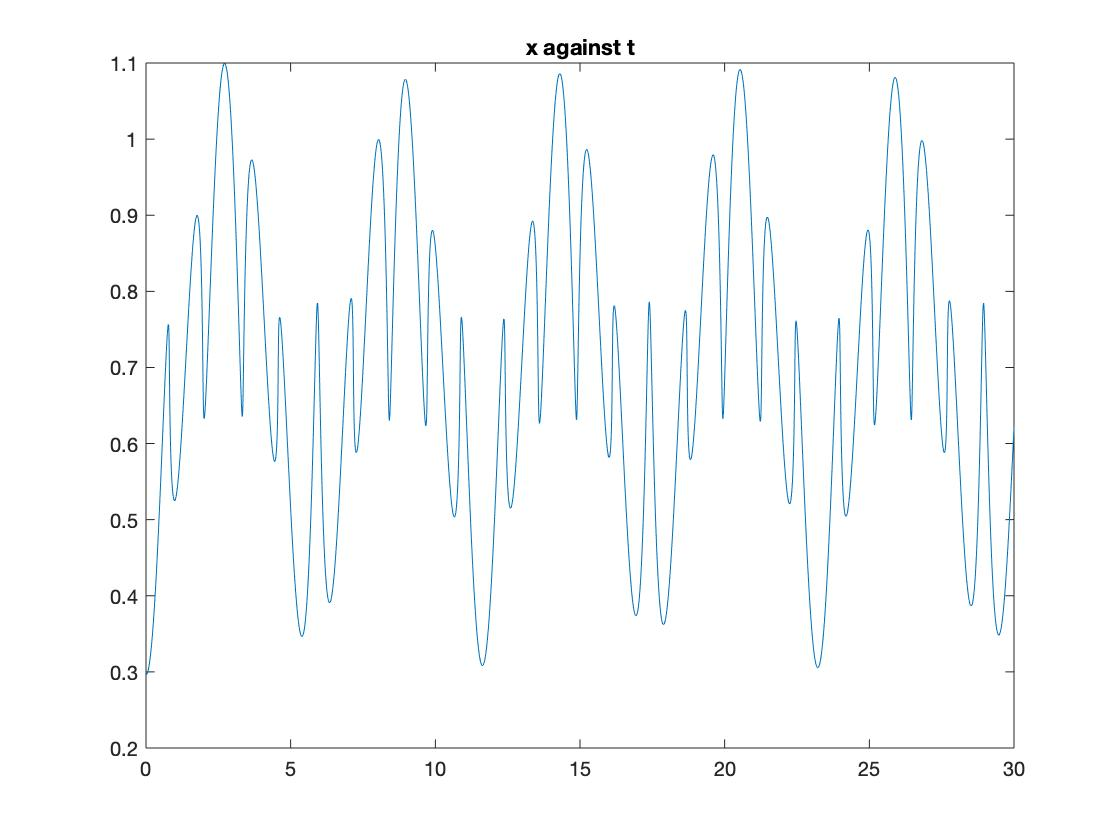
\includegraphics[width = 12cm, height = 8cm]{Q4(7)}
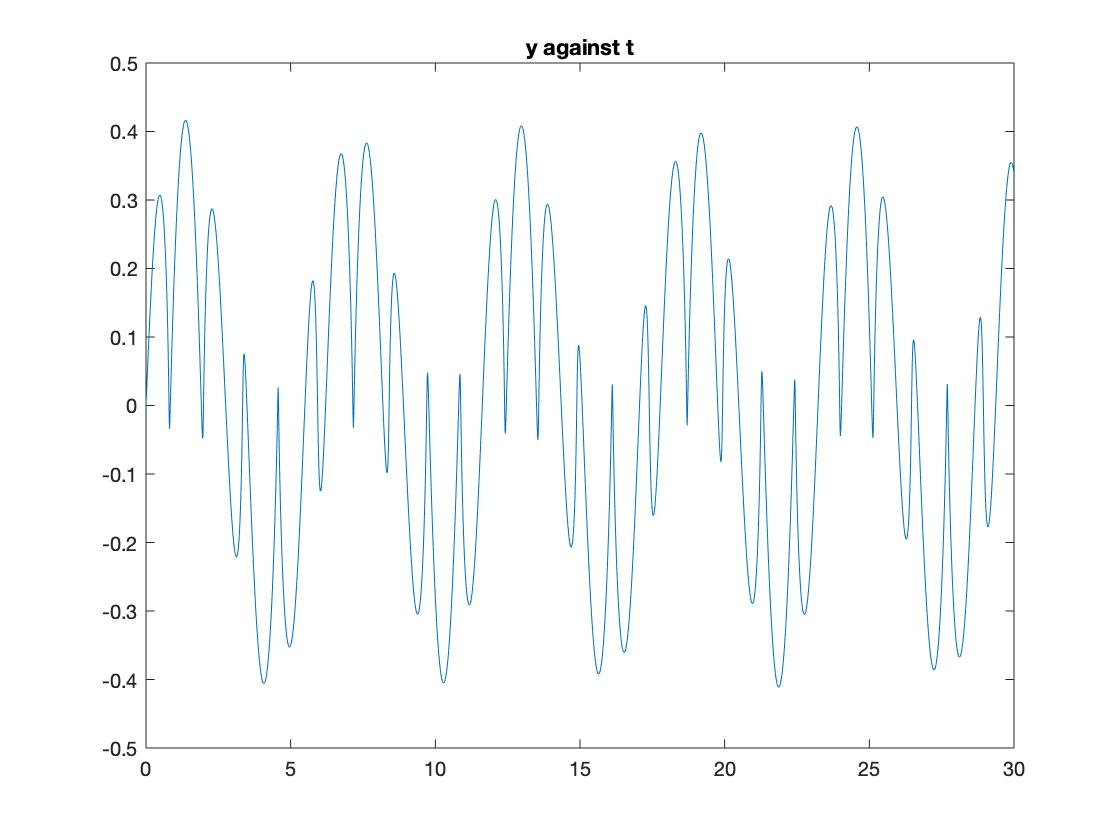
\includegraphics[width = 12cm, height = 8cm]{Q4(8)}
\end{figure}
\begin{figure}[H]
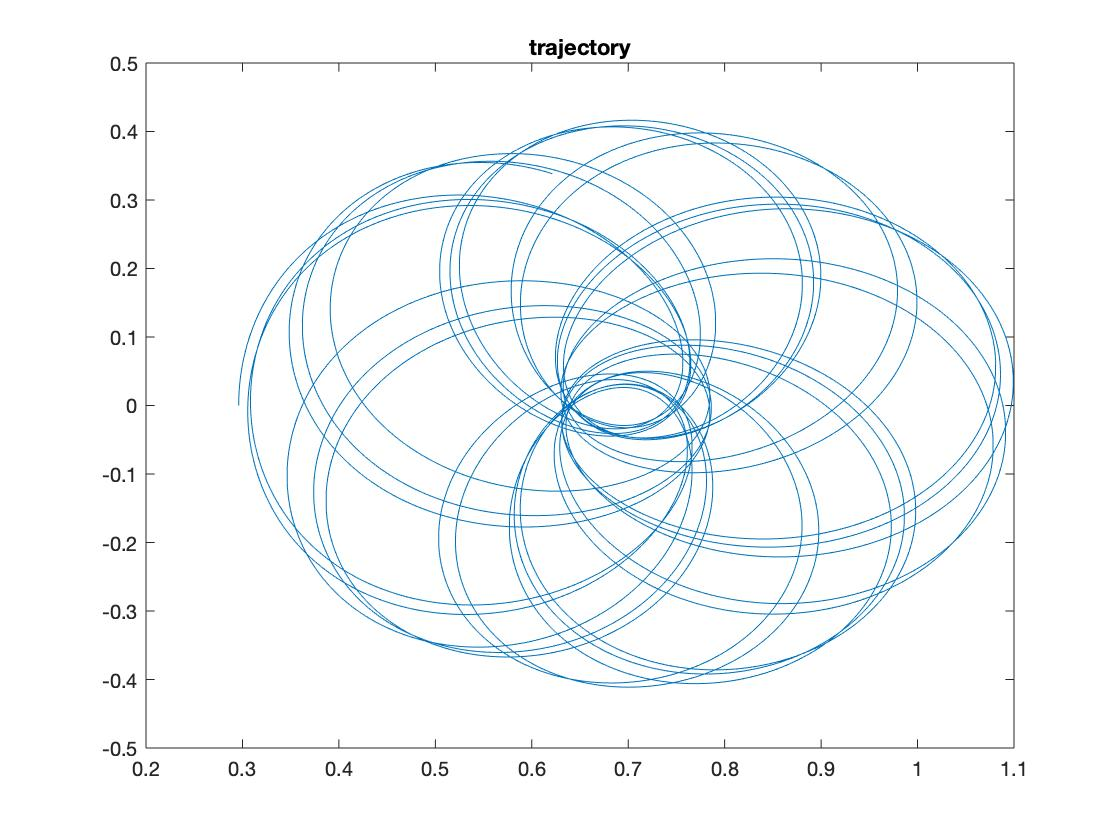
\includegraphics[width = 12cm, height = 8cm]{Q4(9)}
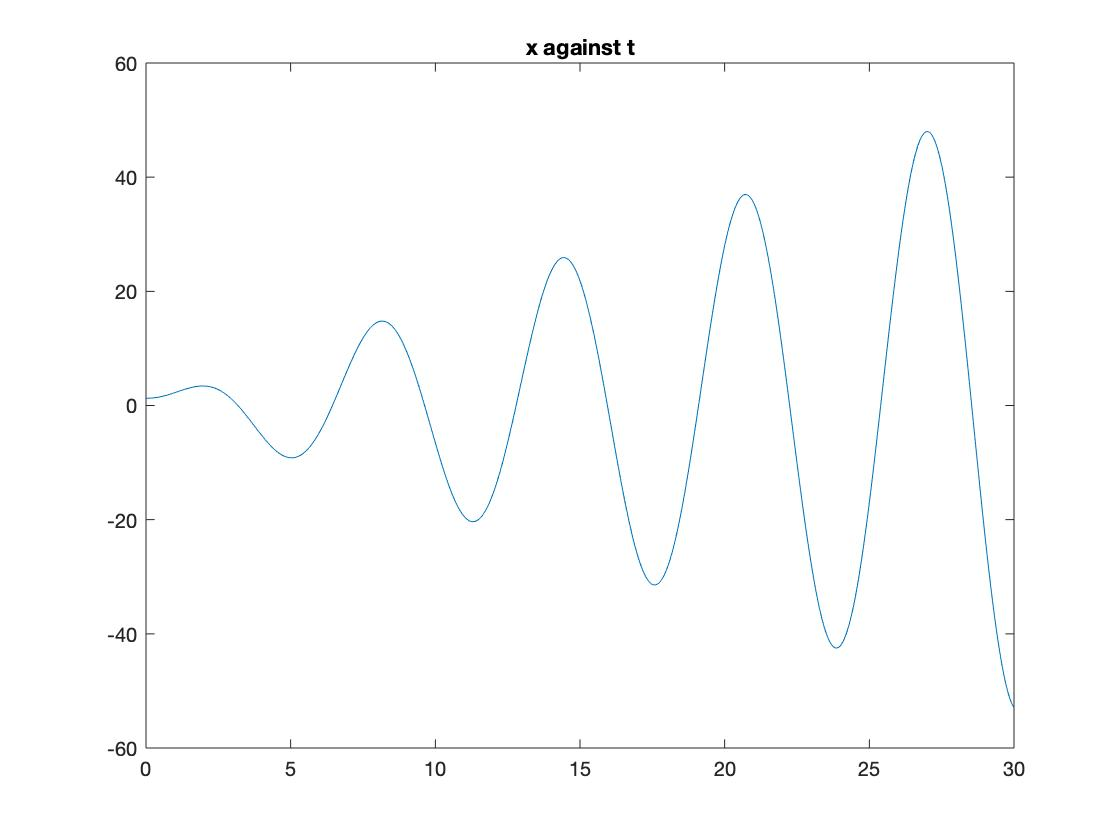
\includegraphics[width = 12cm, height = 8cm]{Q4(10)}
\end{figure}
\begin{figure}[H]
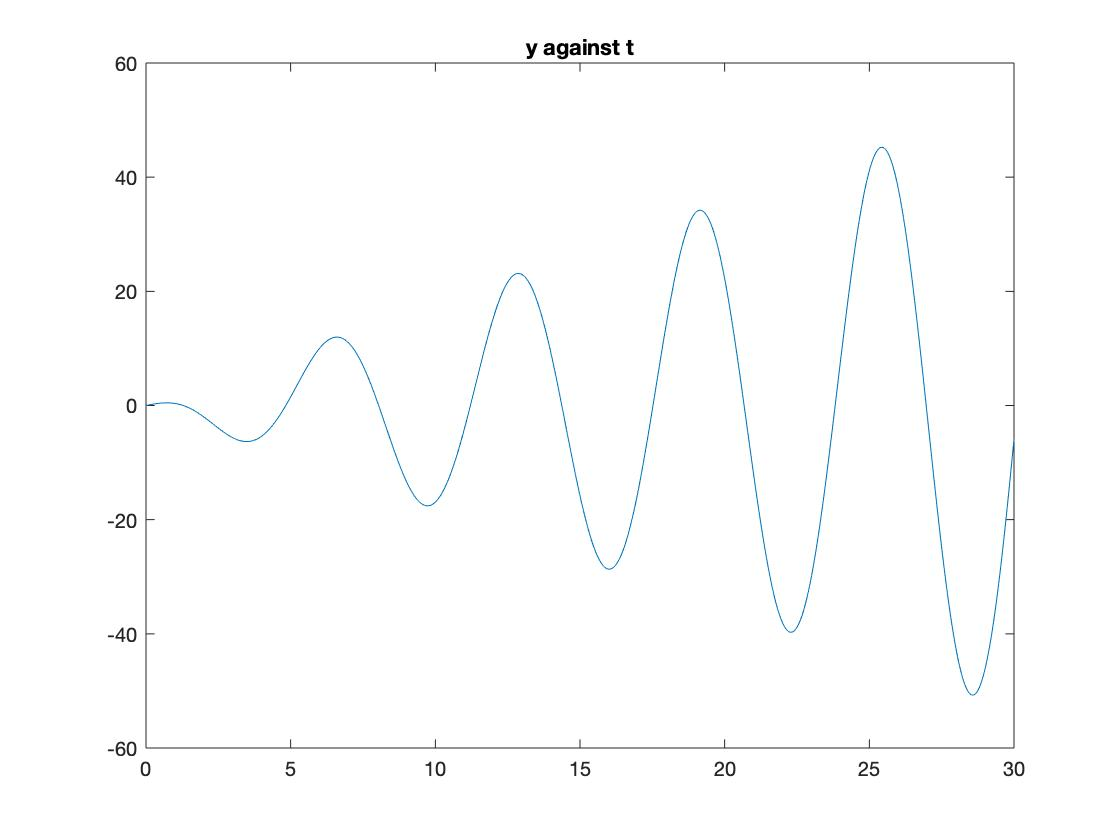
\includegraphics[width = 12cm, height = 8cm]{Q4(11)}
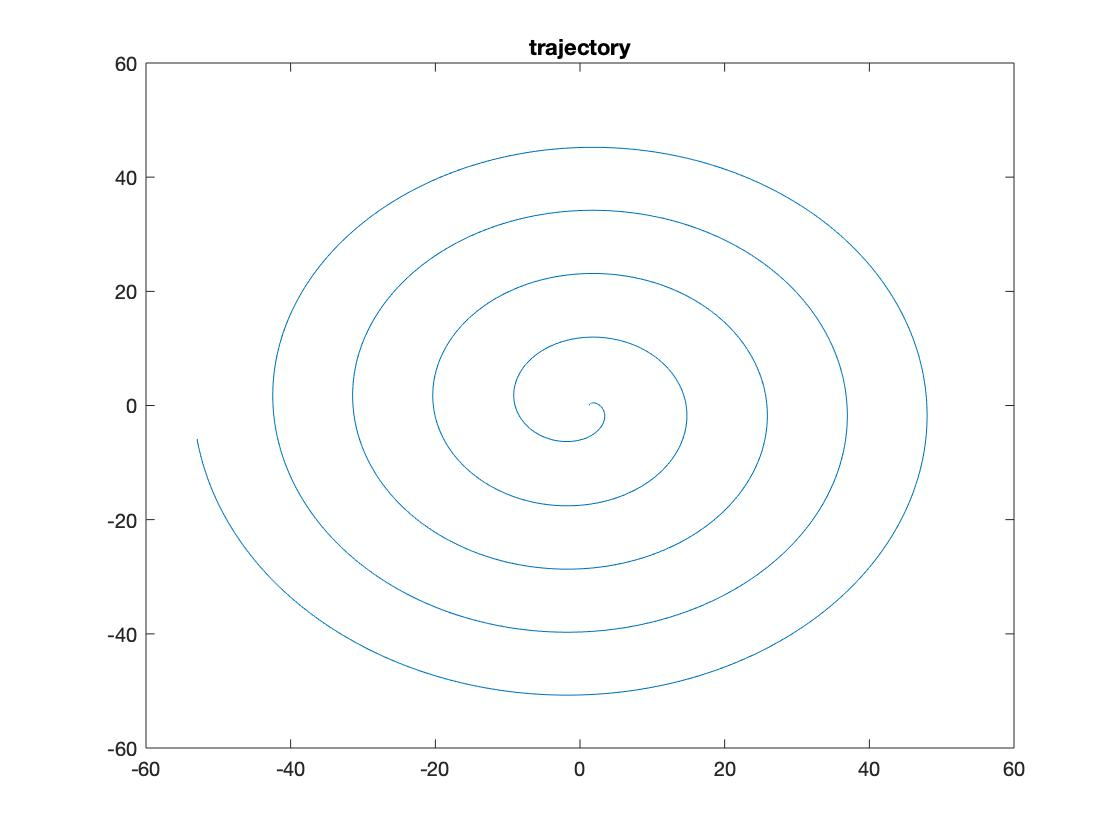
\includegraphics[width = 12cm, height = 8cm]{Q4(12)}
\end{figure}
The first three graphs show the positions of five Lagrange points and contours of $\Omega > J$ for different values of $\mu$( here i took $\Omega>J$ as it is not evident to draw a contour graph for all values of $\Omega$, as they differ only by a little ), and the 9 following show the evolution of x against t , y against t, and the trajectories of the third body starting near the collinear Lagrange points, with a perturbation of 0.01. It is evident from the diagrams that the collinear lagrange points are unstable. From the contours of $\Omega$ we can observe that the collinear Lagrange points are saddle points, and hence they must be unstable, no matter how big $\mu$ is. To perform the linearised analysis, we need to check the Hessian of $\Omega$ and find out its eigenvalues. The contour plot has shown that it must have eigenvalues of distinct signs, hence unstable.
\subsection{Question 5}
The graphs below are as requested by the question. The stability of Equilateral Lagrange points seems to be weakened as $\mu$ increases.
\newpage
\begin{figure}[H]
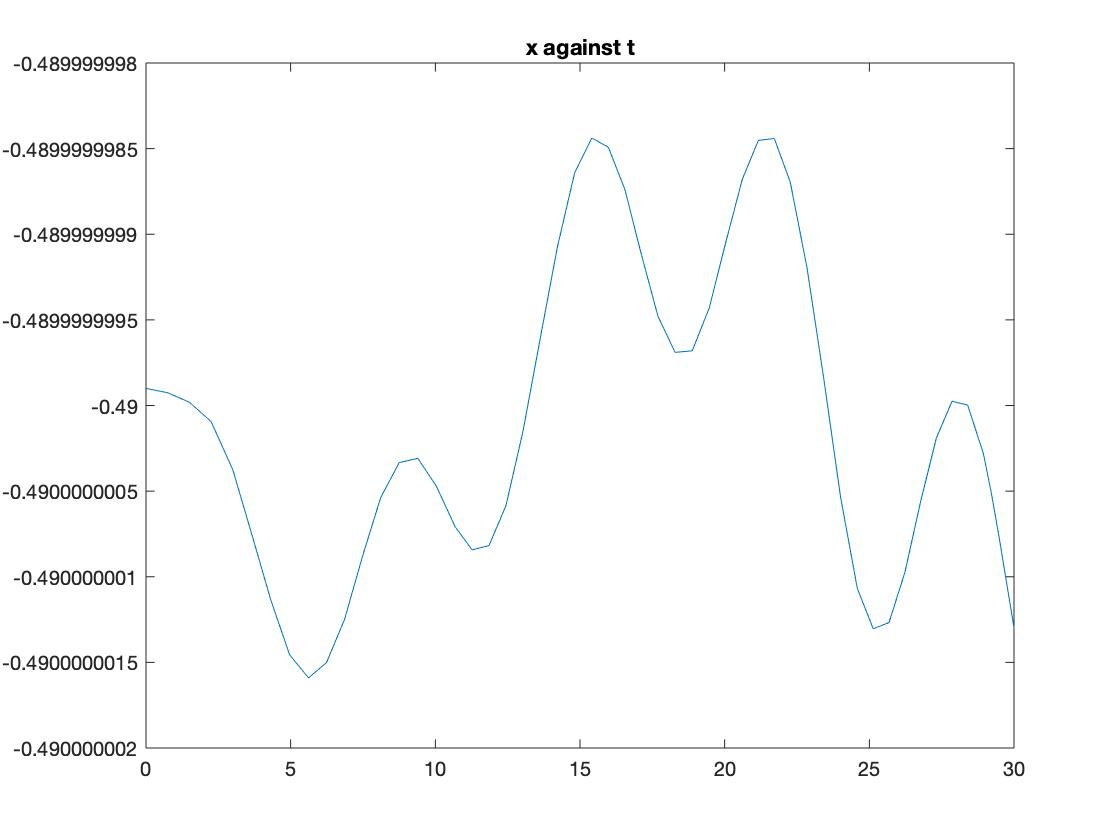
\includegraphics[width = 12cm, height = 8cm]{Q5(1).jpg}
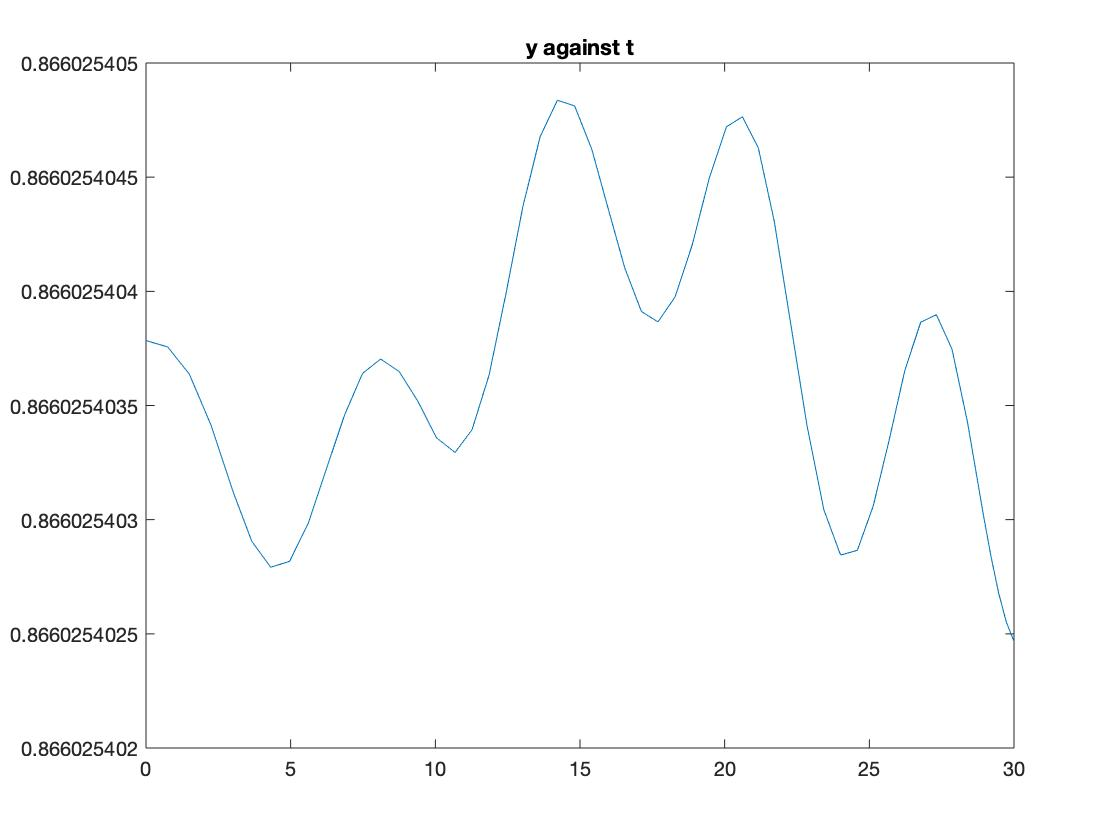
\includegraphics[width = 12cm, height = 8cm]{Q5(2).jpg}
\end{figure}
\begin{figure}[H]
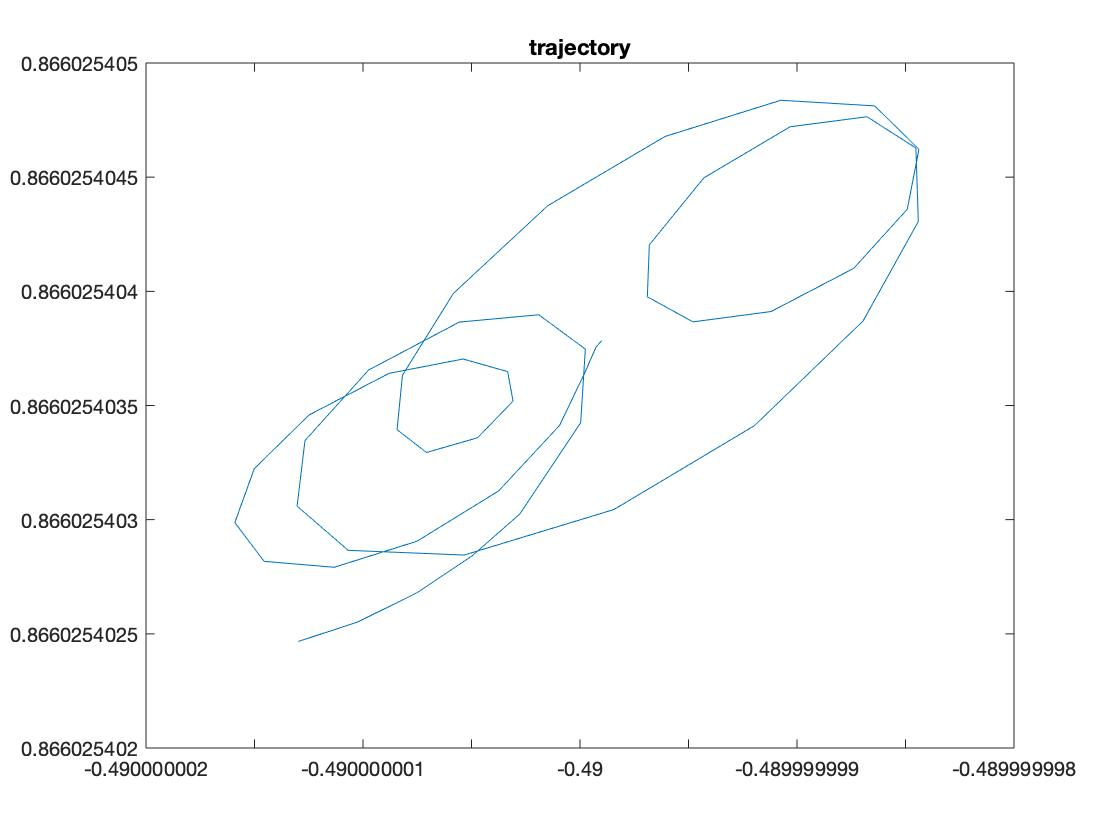
\includegraphics[width = 12cm, height = 8cm]{Q5(3).jpg}
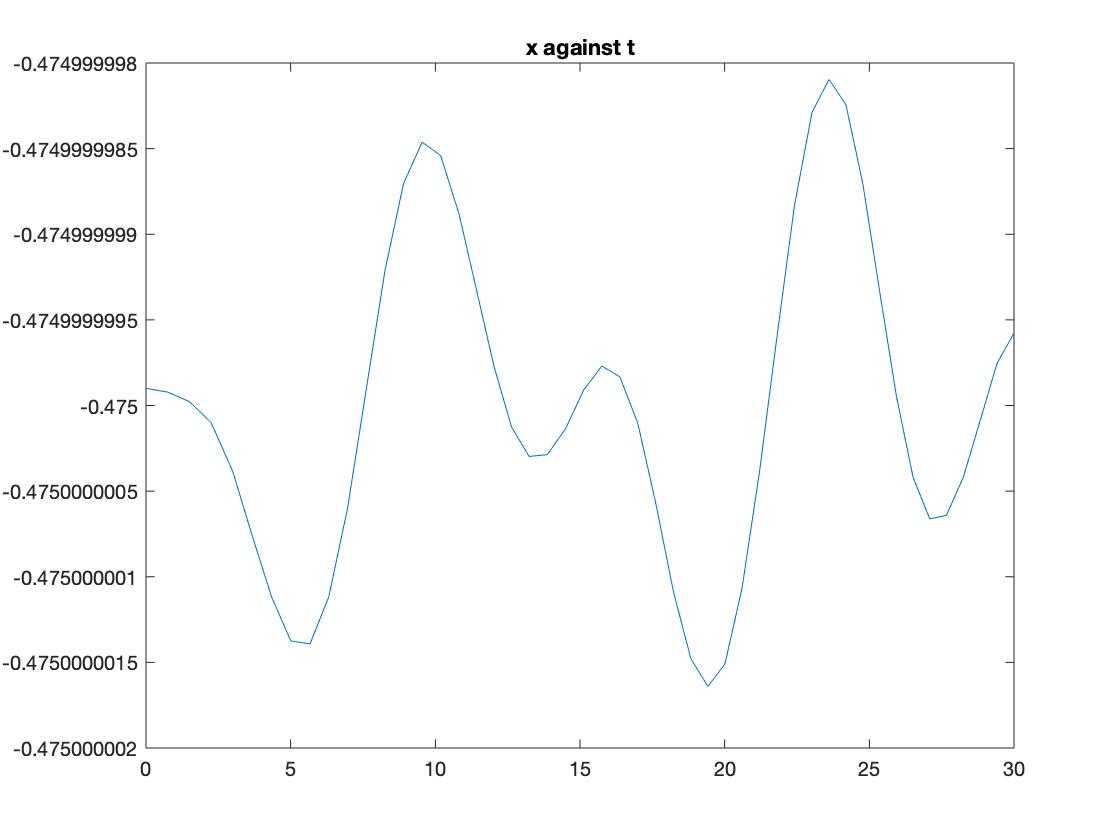
\includegraphics[width = 12cm, height = 8cm]{Q5(4).jpg}
\end{figure}
\begin{figure}[H]
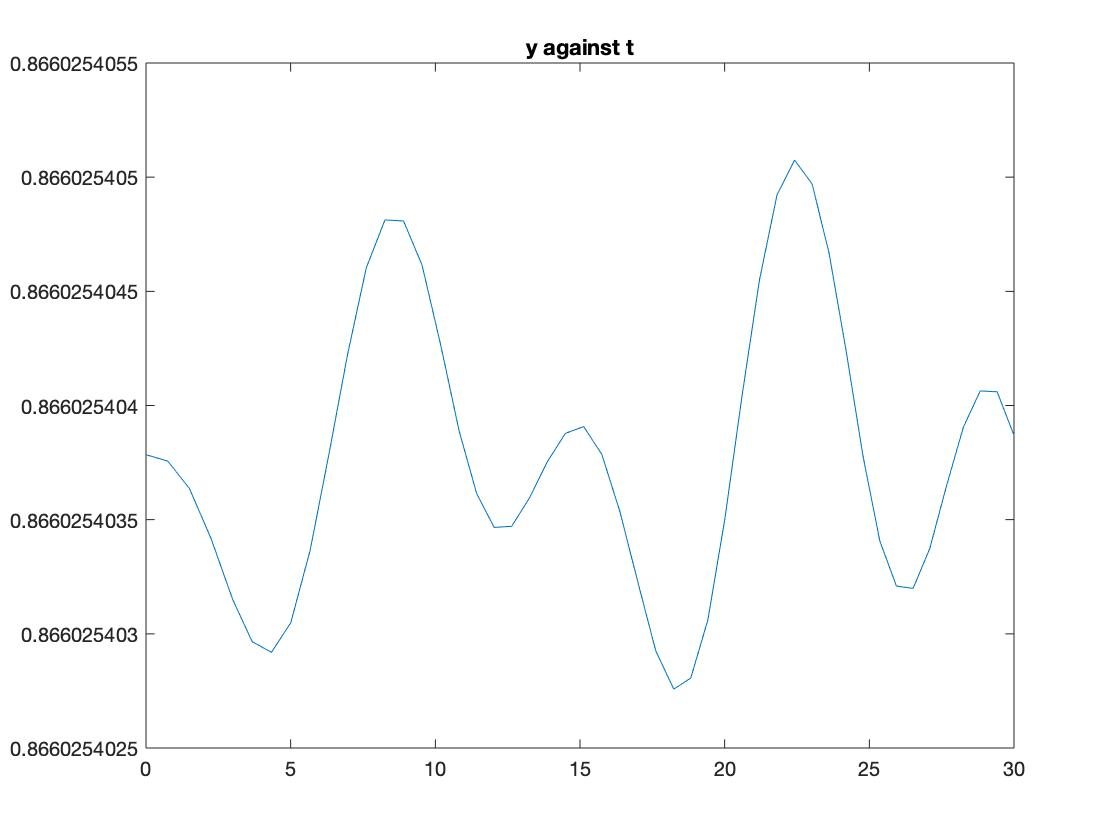
\includegraphics[width = 12cm, height = 8cm]{Q5(5).jpg}
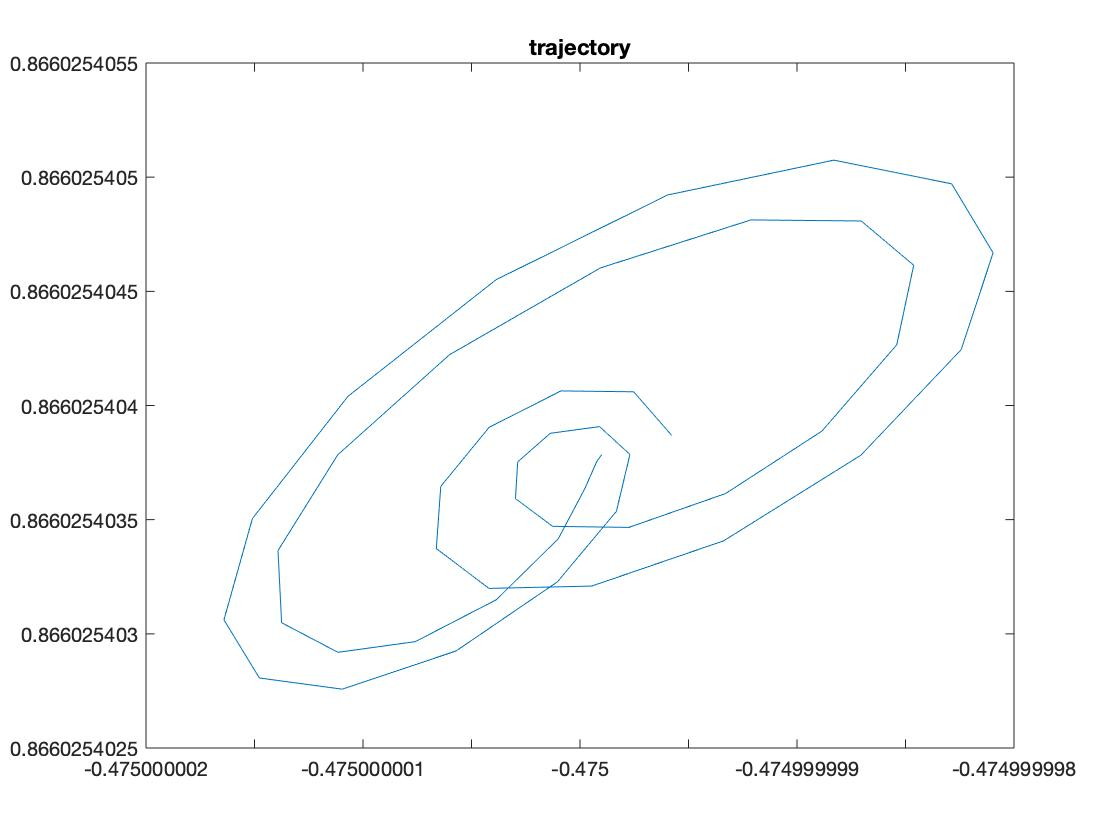
\includegraphics[width = 12cm, height = 8cm]{Q5(6).jpg}
\end{figure}
\begin{figure}[H]
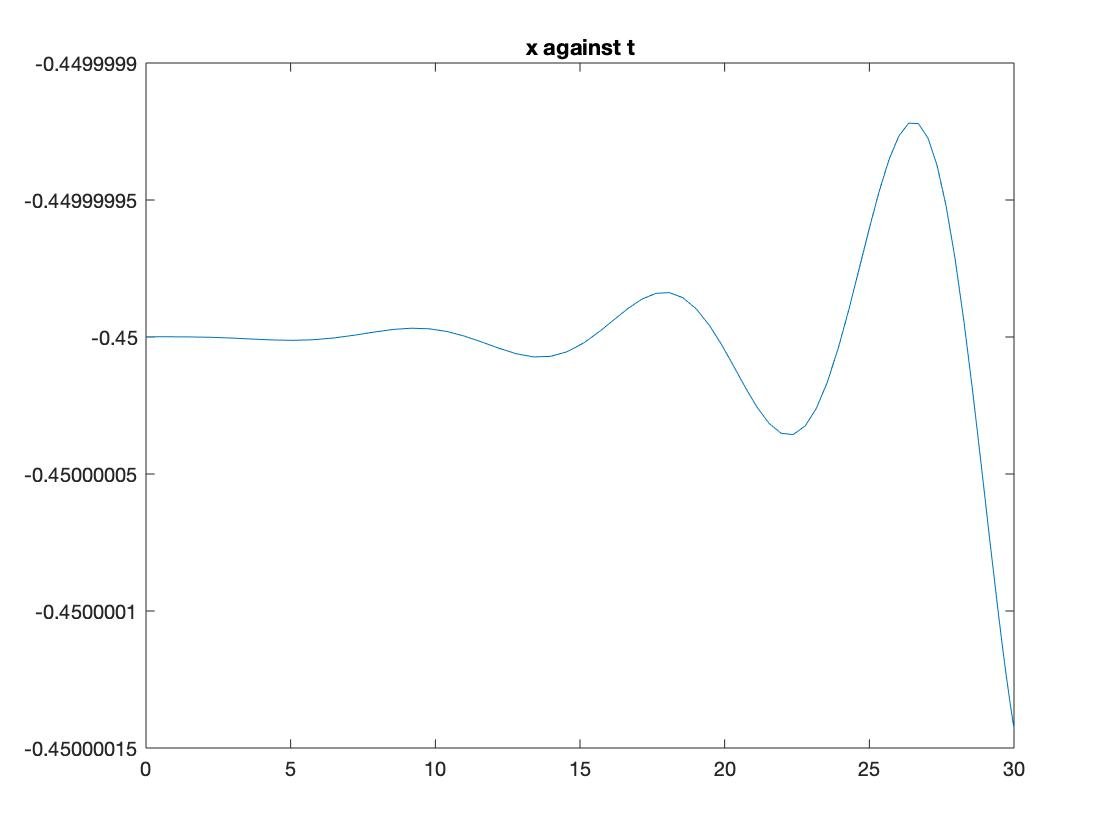
\includegraphics[width = 12cm, height = 8cm]{Q5(7).jpg}
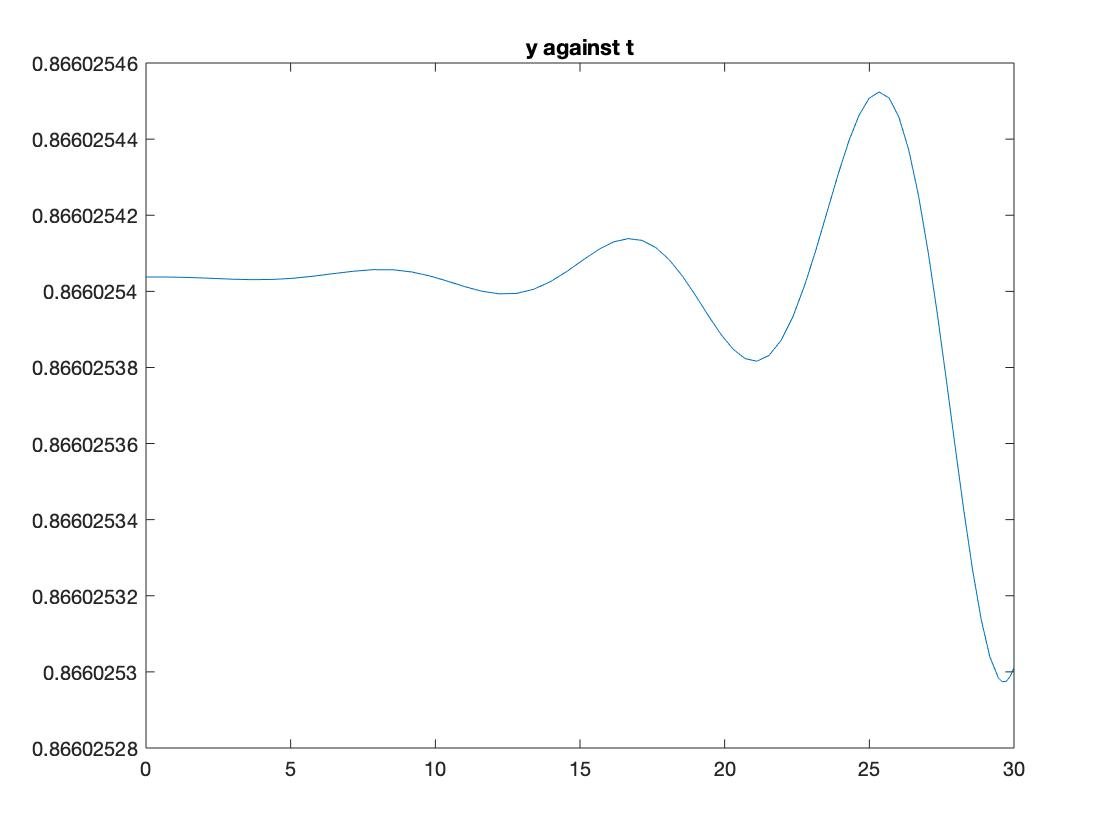
\includegraphics[width = 12cm, height = 8cm]{Q5(8).jpg}
\end{figure}
\begin{figure}[H]
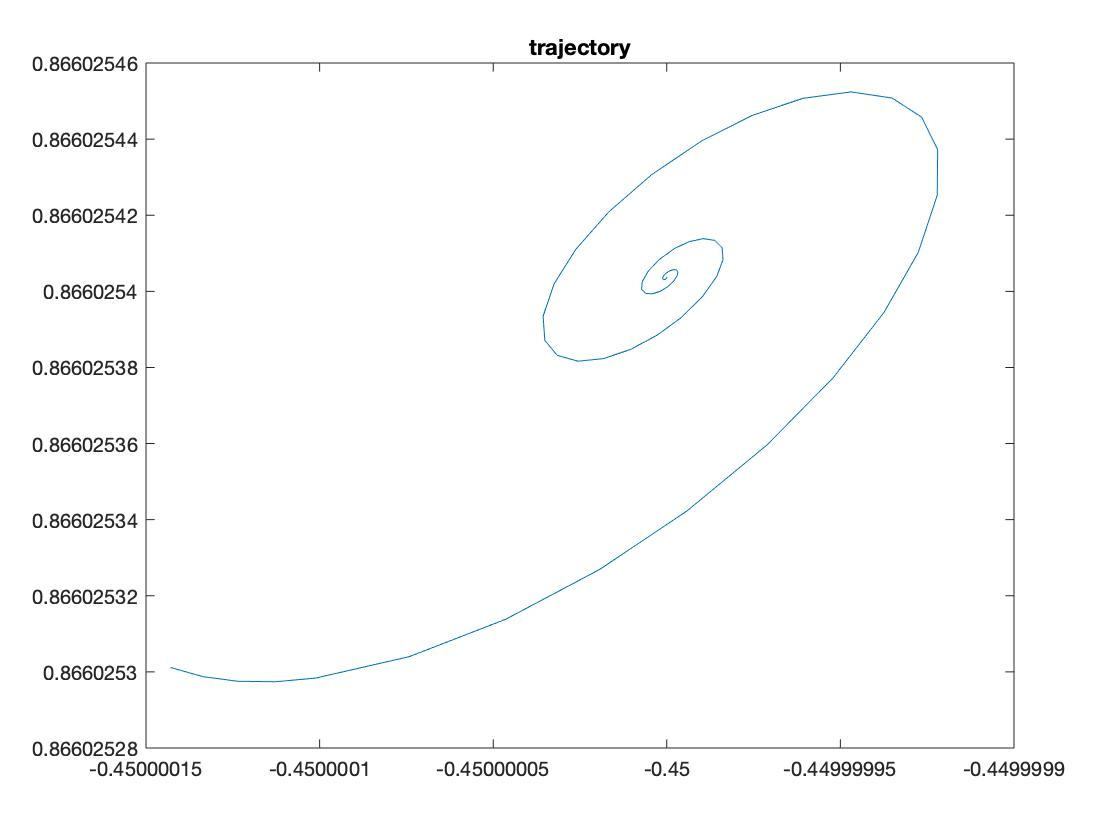
\includegraphics[width = 12cm, height = 8cm]{Q5(9).jpg}
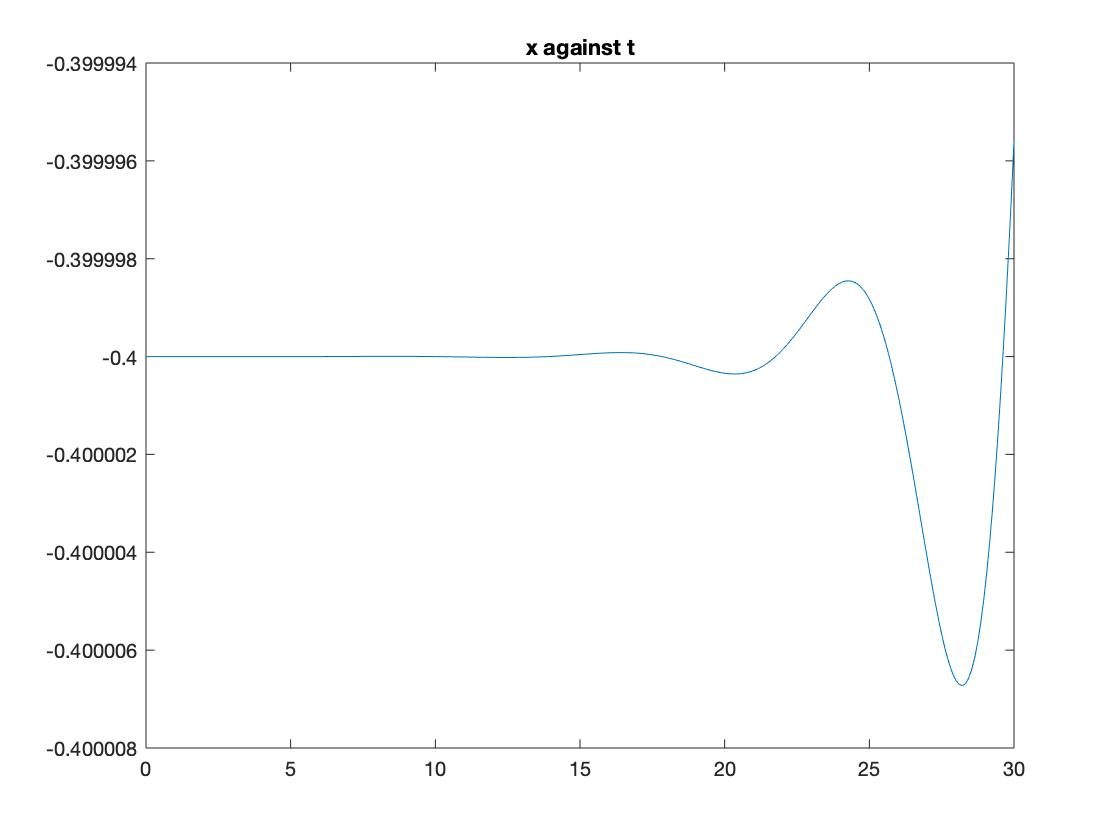
\includegraphics[width = 12cm, height = 8cm]{Q5(10).jpg}
\end{figure}
\begin{figure}[H]
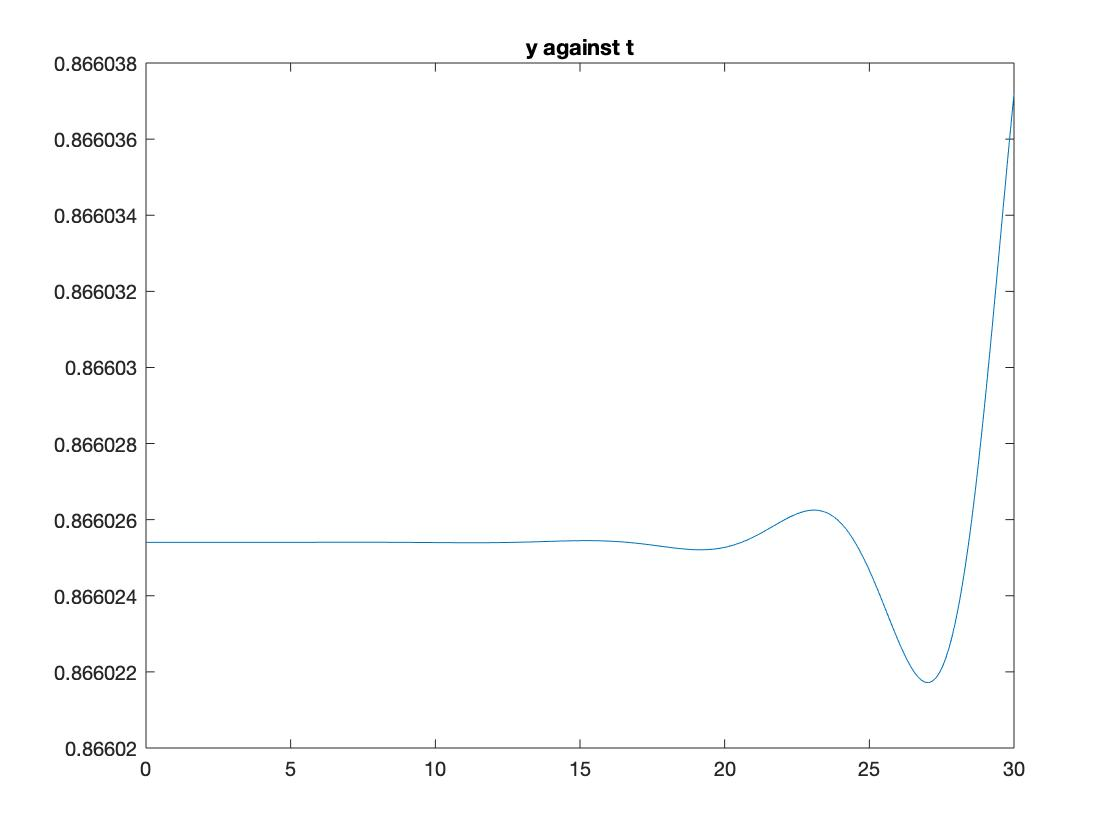
\includegraphics[width = 12cm, height = 8cm]{Q5(11).jpg}
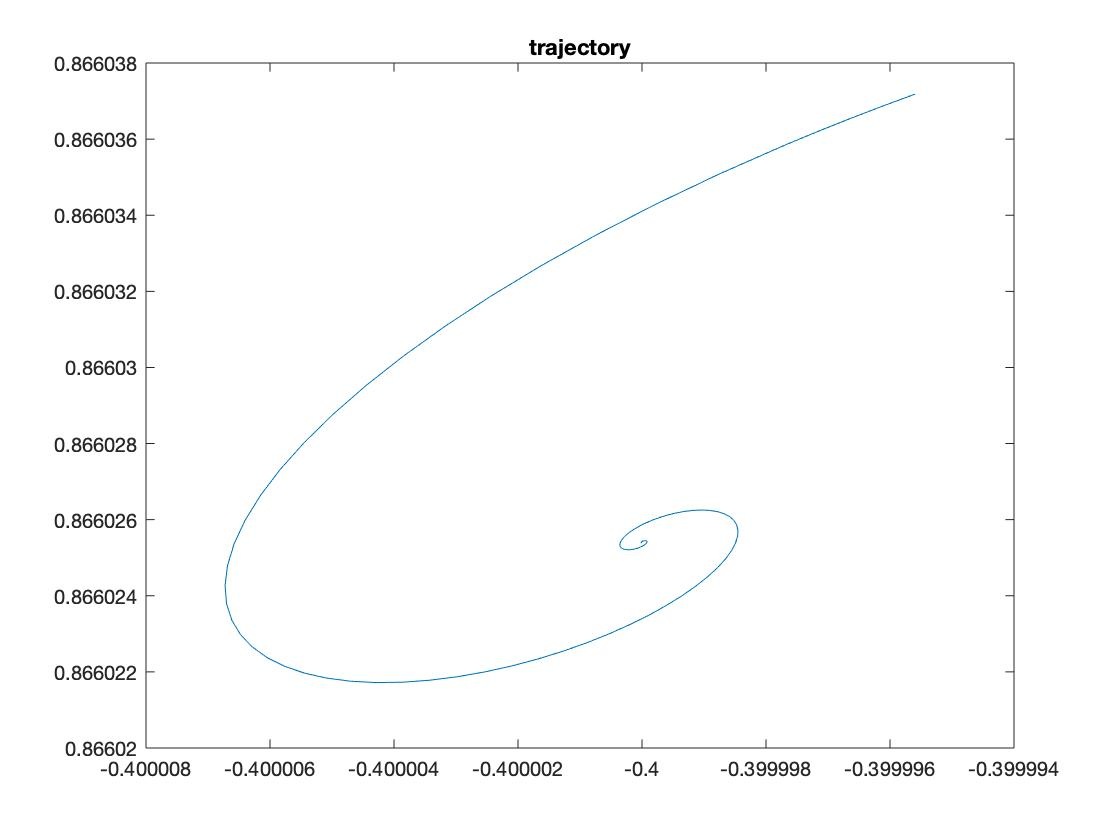
\includegraphics[width = 12cm, height = 8cm]{Q5(12).jpg}
\end{figure}
\begin{figure}[H]
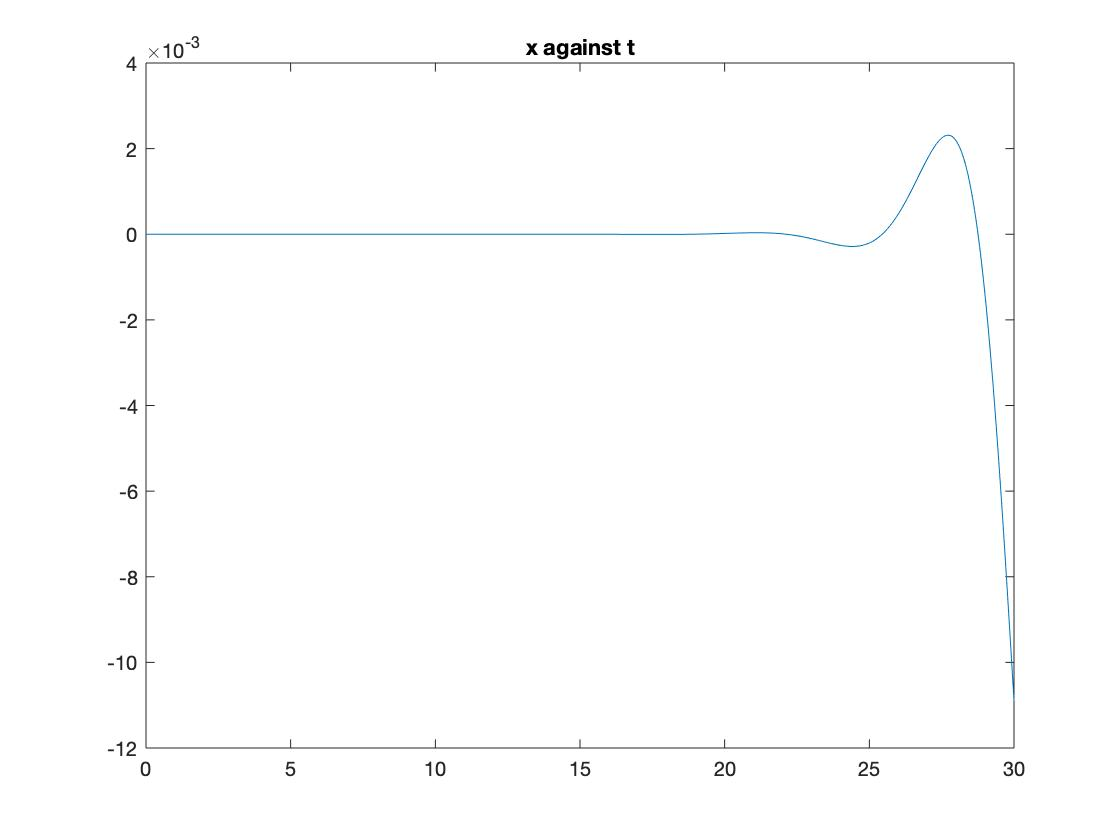
\includegraphics[width = 12cm, height = 8cm]{Q5(13).jpg}
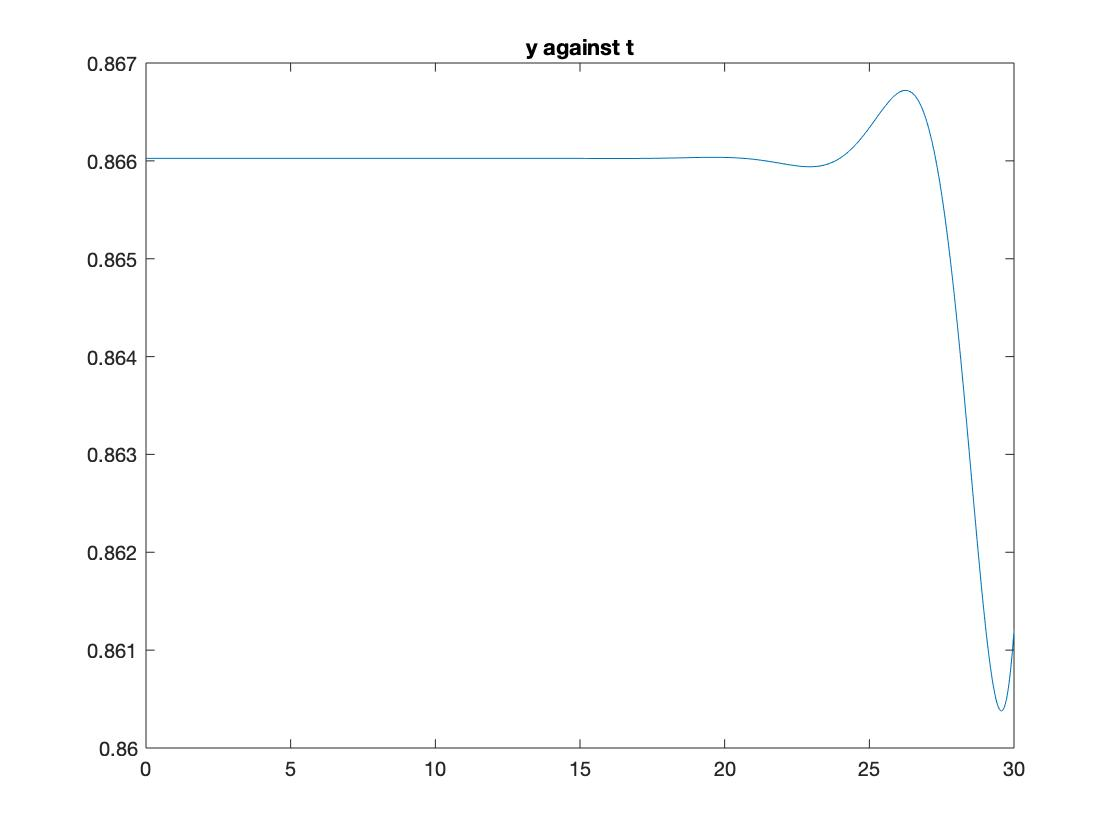
\includegraphics[width = 12cm, height = 8cm]{Q5(14).jpg}
\end{figure}
\begin{figure}[H]
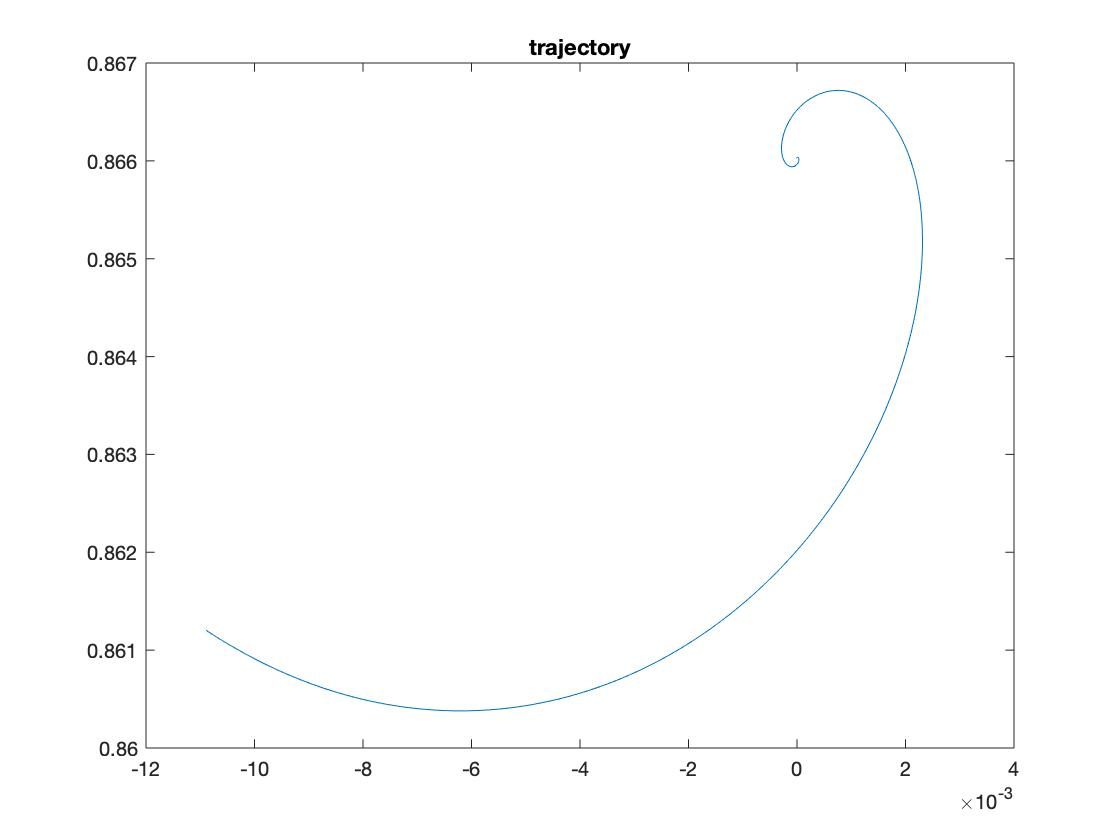
\includegraphics[width = 12cm, height = 8cm]{Q5(15).jpg}
\end{figure}
\newpage
We then do further numerical investigation from 0.02 to 0.05, with step size of 0.01.From below you can see that $\mu_{c} \in (0.03,0.04)$
\begin{figure}[H]
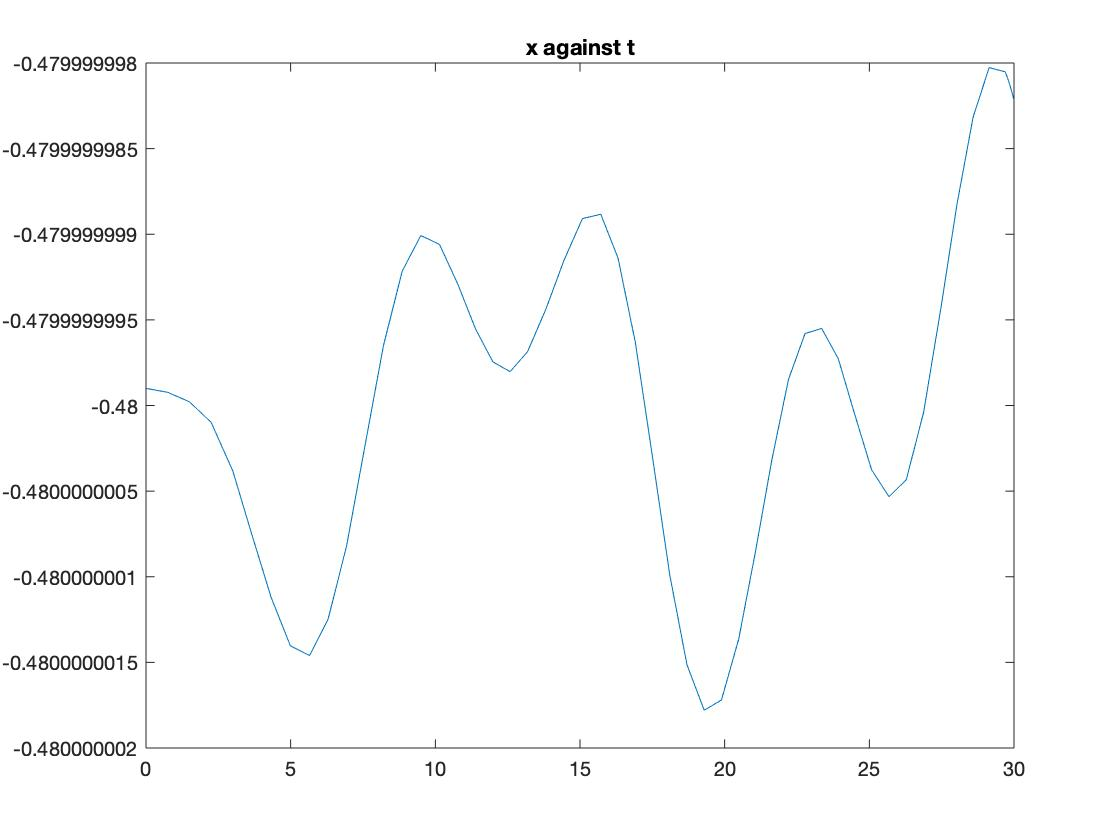
\includegraphics[width = 12cm, height = 8cm]{Q5(16).jpg}
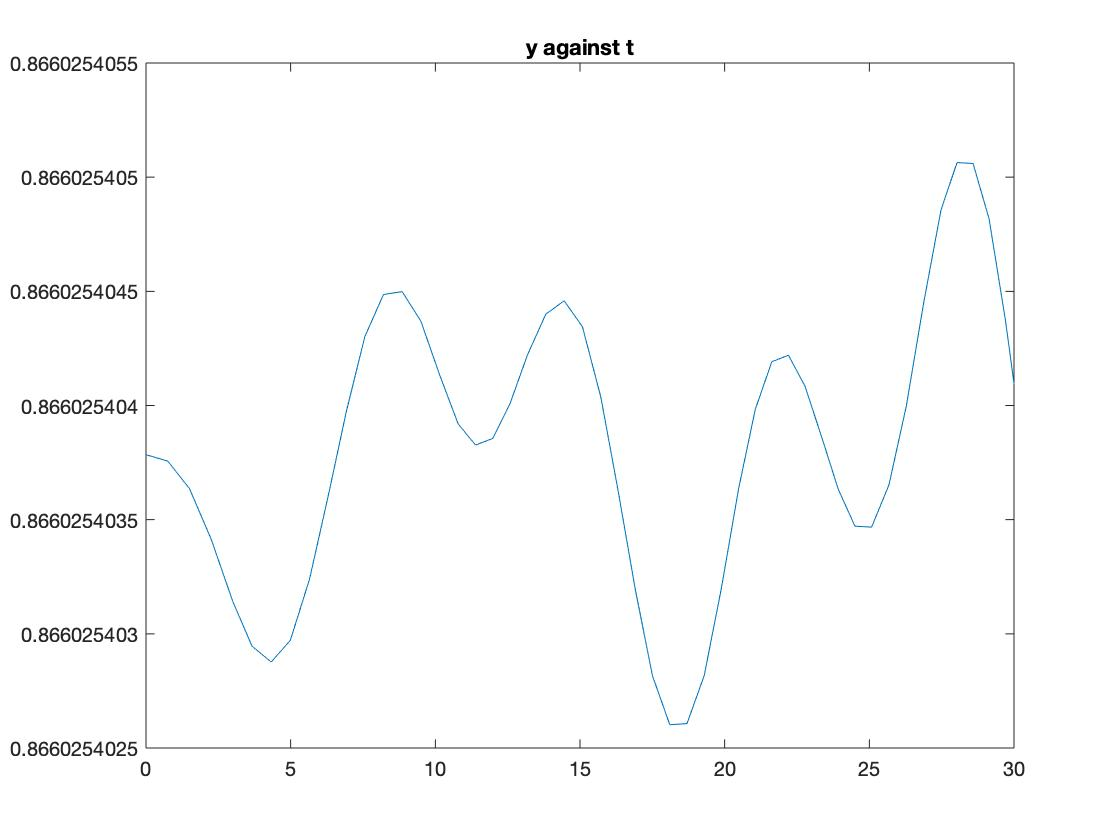
\includegraphics[width = 12cm, height = 8cm]{Q5(17).jpg}
\end{figure}
\begin{figure}[H]
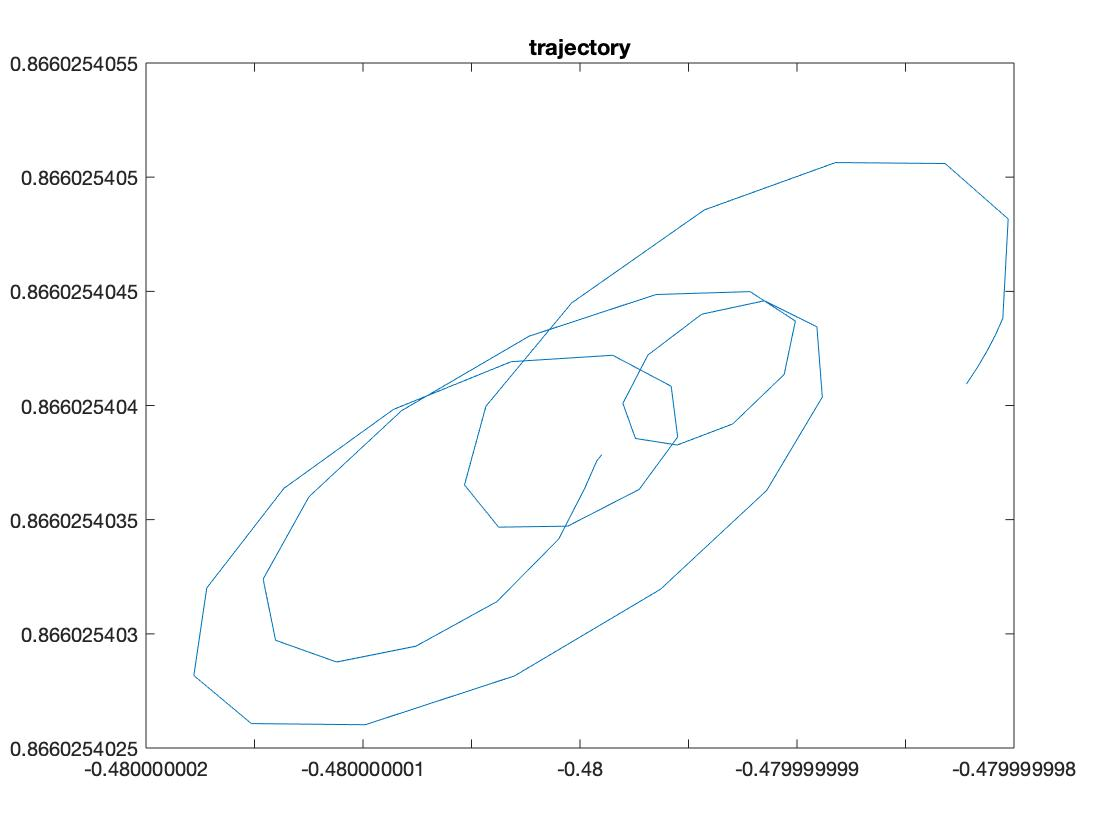
\includegraphics[width = 12cm, height = 8cm]{Q5(18).jpg}\\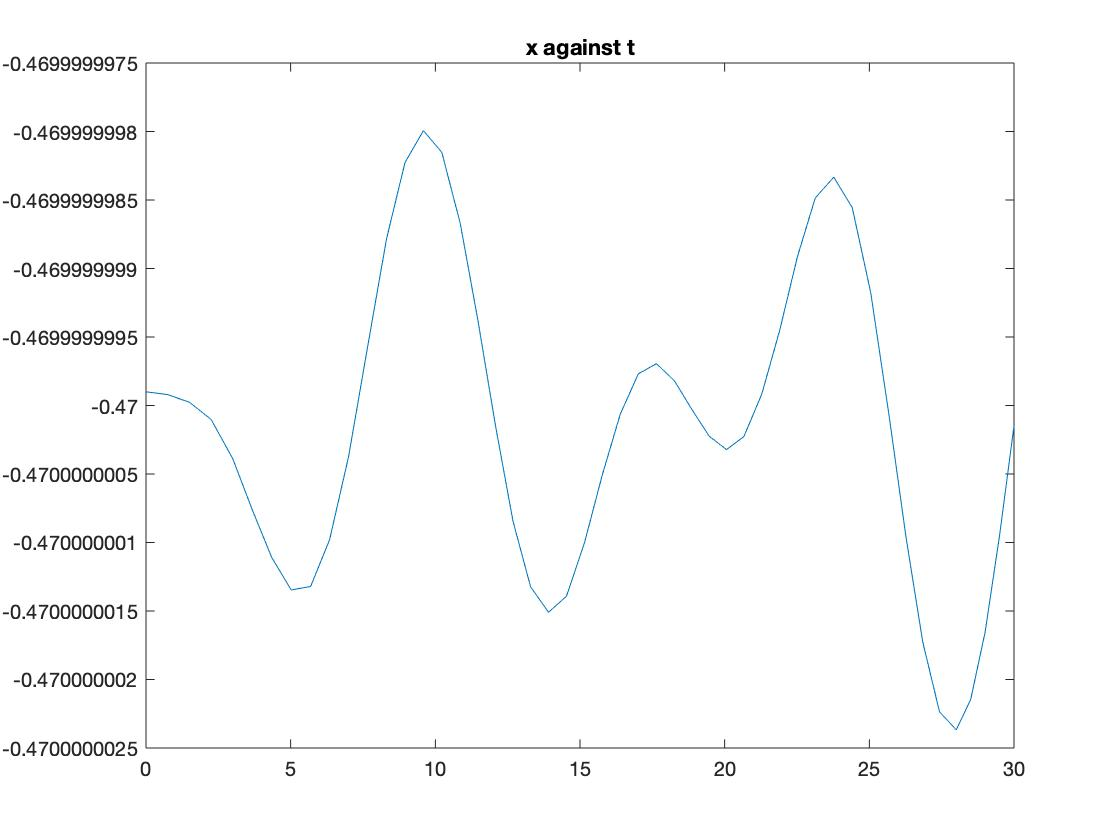
\includegraphics[width = 12cm, height = 8cm]{Q5(19).jpg}
\end{figure}
\begin{figure}[H]
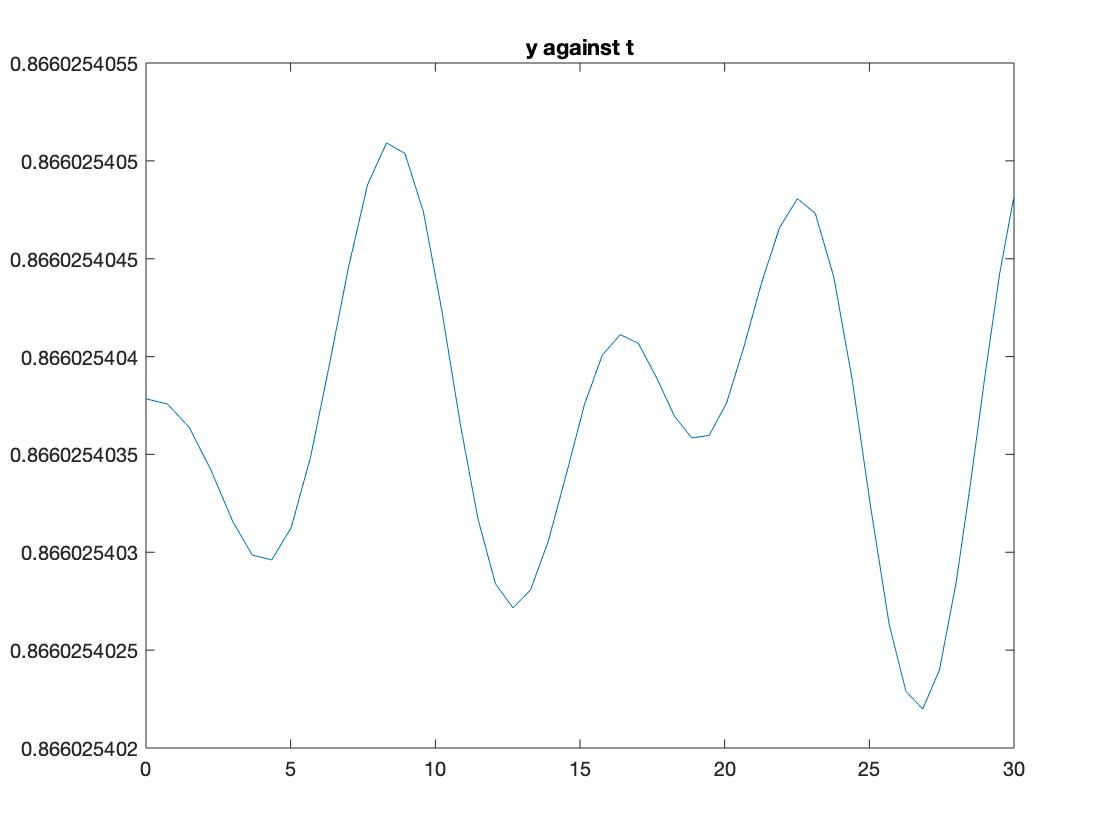
\includegraphics[width = 12cm, height = 8cm]{Q5(20).jpg}
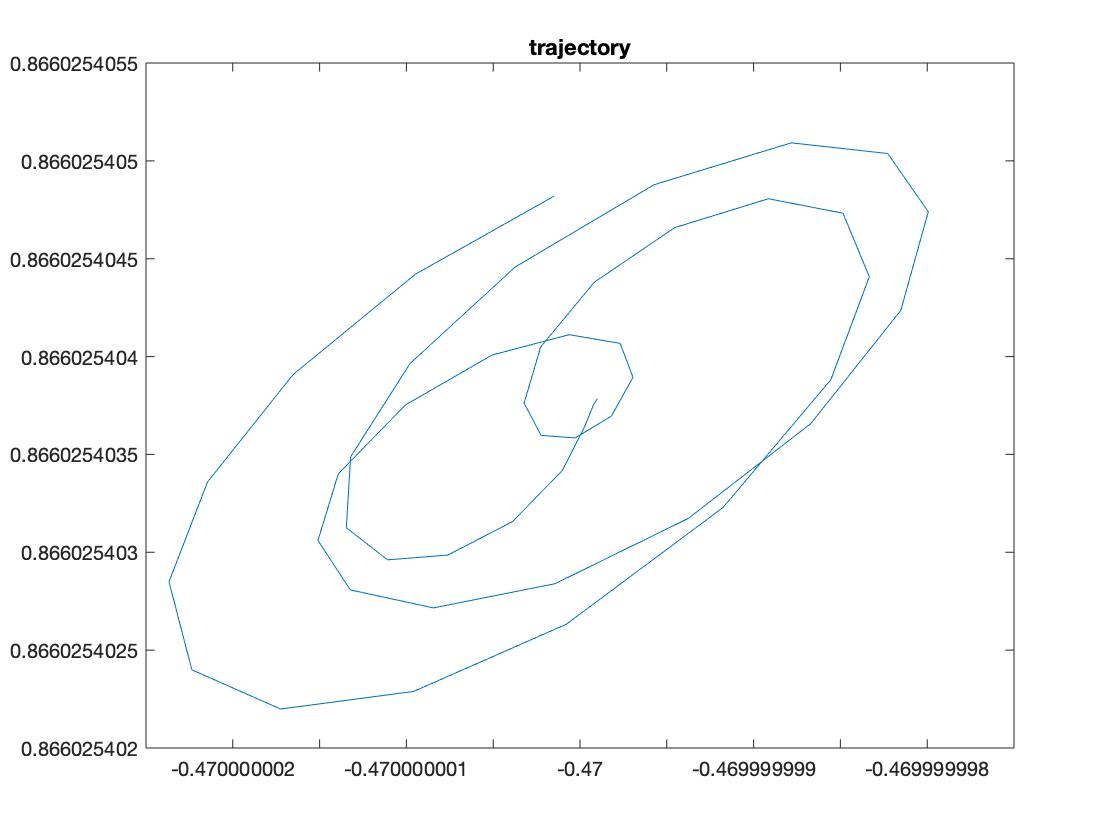
\includegraphics[width = 12cm, height = 8cm]{Q5(21).jpg}
\end{figure}
\begin{figure}[H]
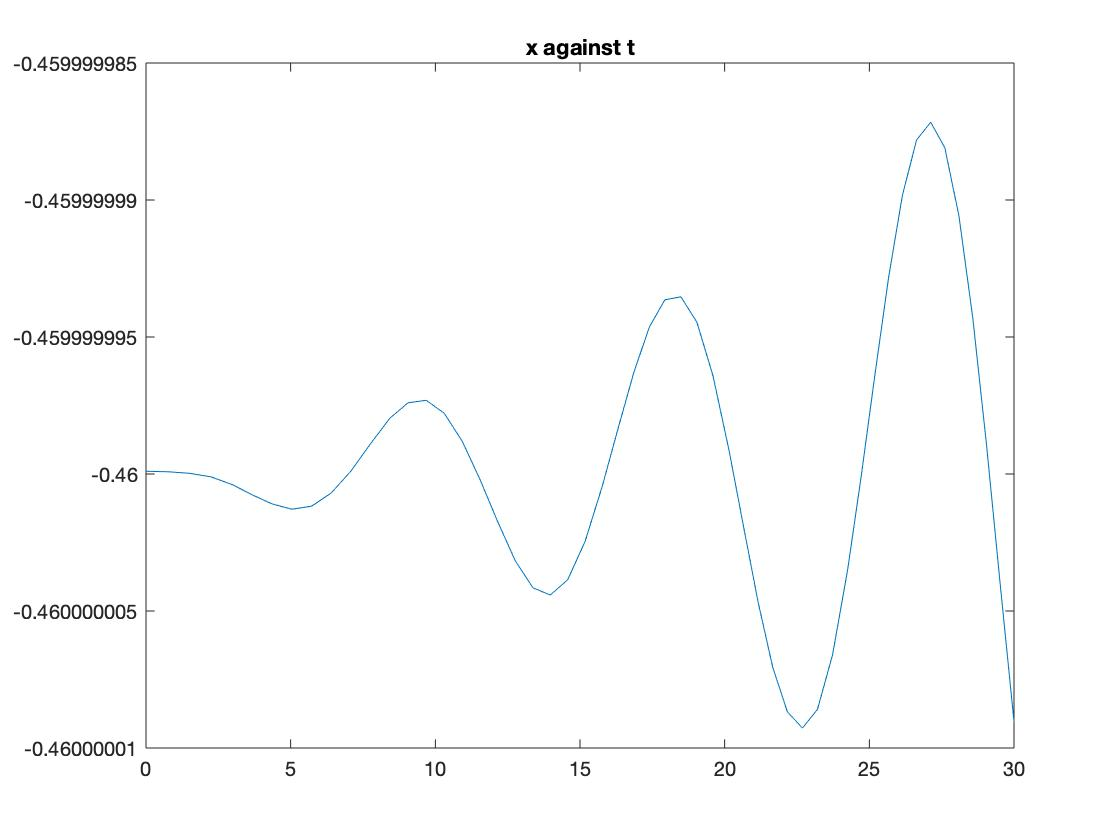
\includegraphics[width = 12cm, height = 8cm]{Q5(22).jpg}\\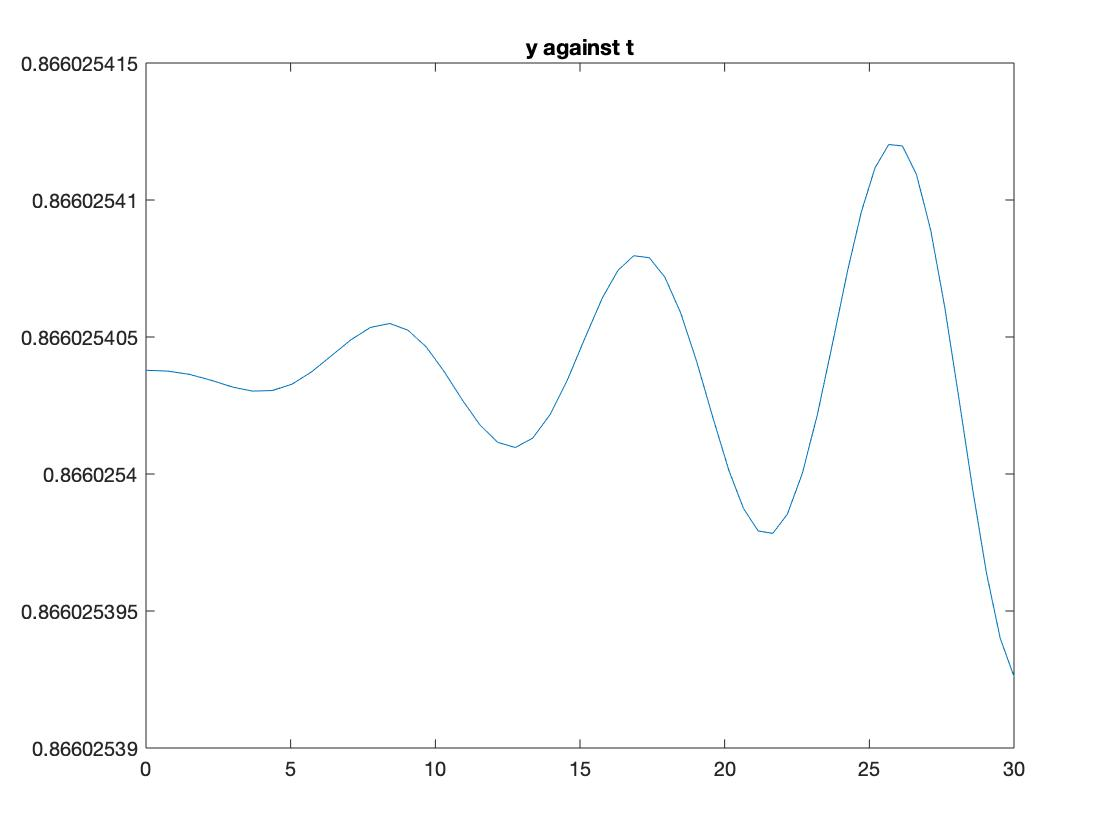
\includegraphics[width = 12cm, height = 8cm]{Q5(23).jpg}
\end{figure}
\begin{figure}[H]
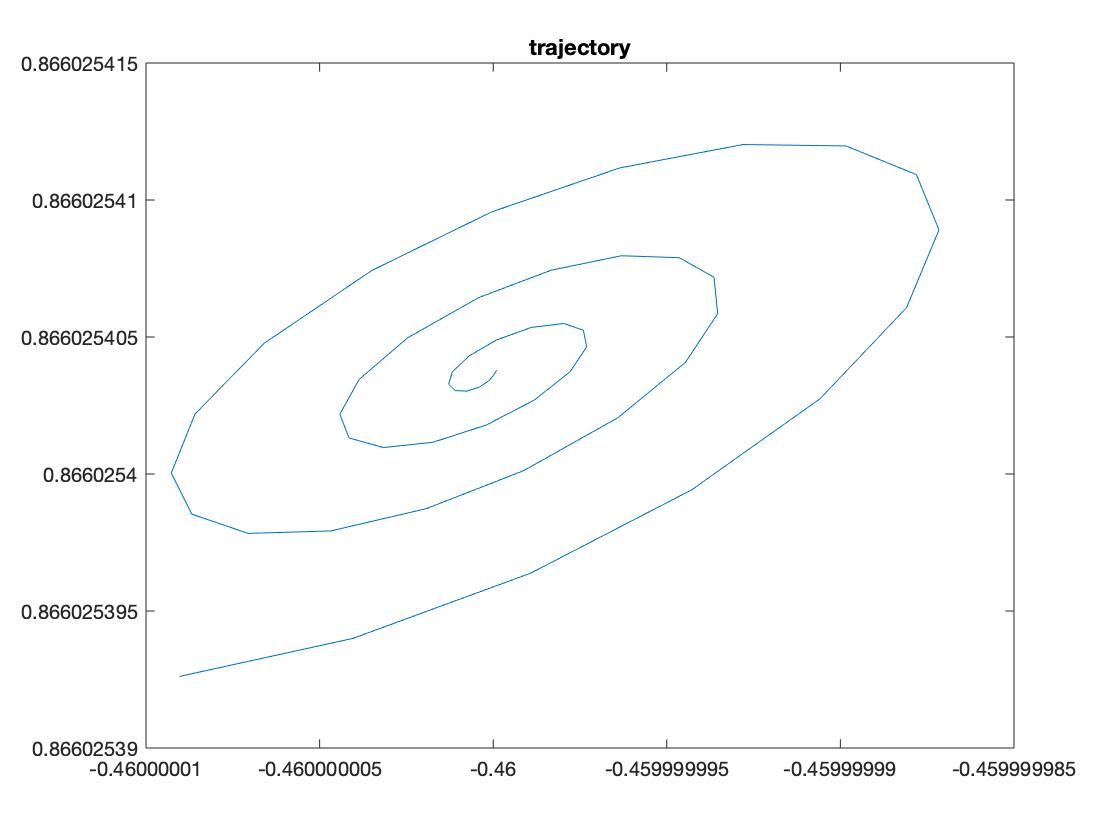
\includegraphics[width = 12cm, height = 8cm]{Q5(24).jpg}
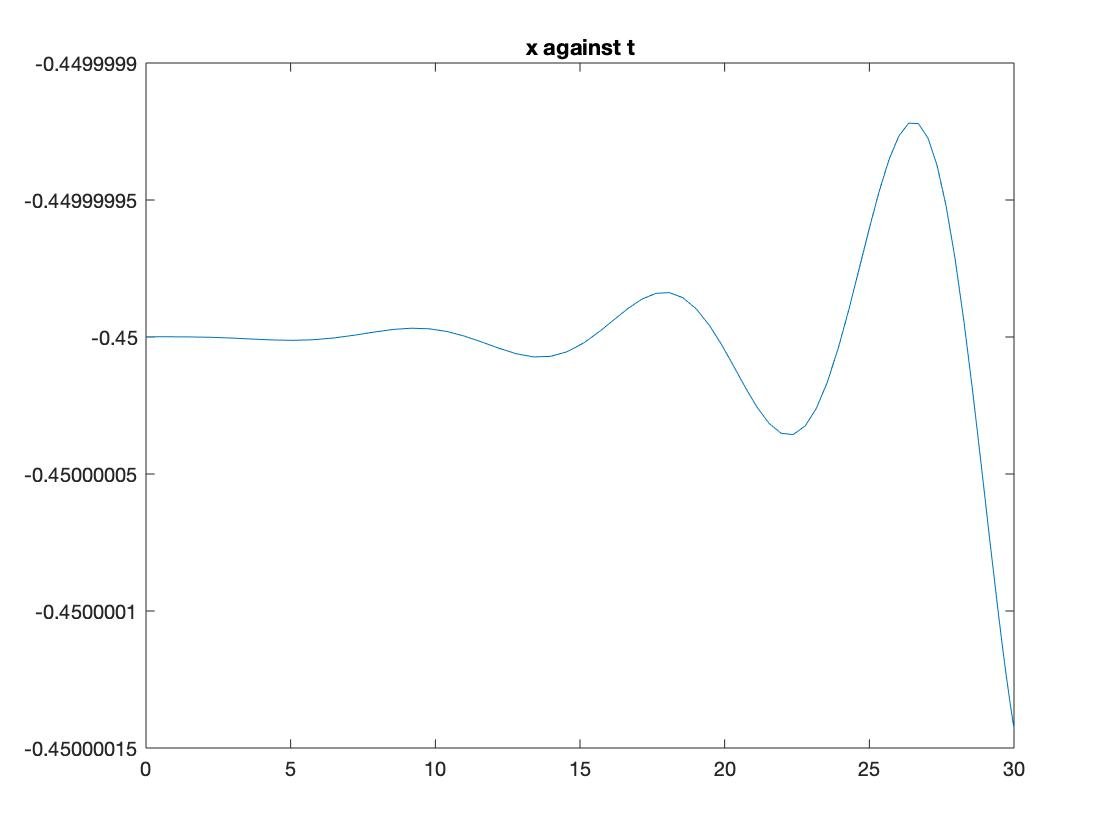
\includegraphics[width = 12cm, height = 8cm]{Q5(25).jpg}
\end{figure}
\begin{figure}[H]
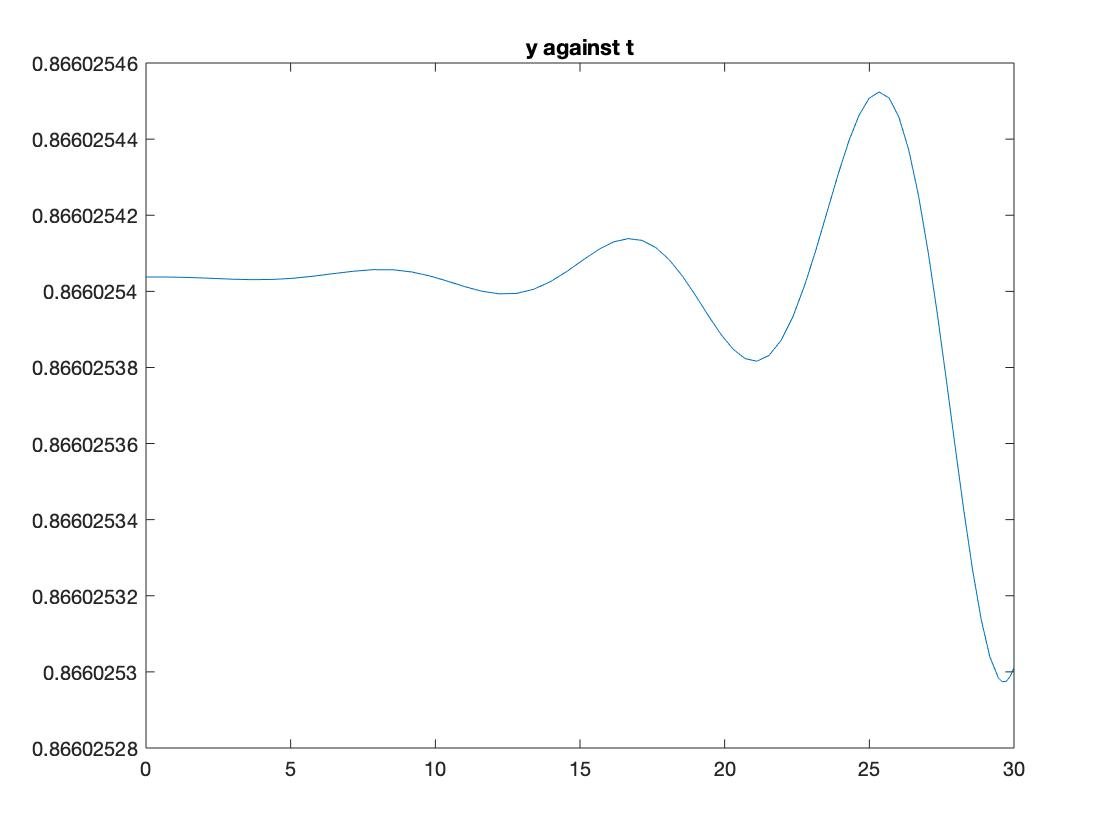
\includegraphics[width = 12cm, height = 8cm]{Q5(26).jpg}\\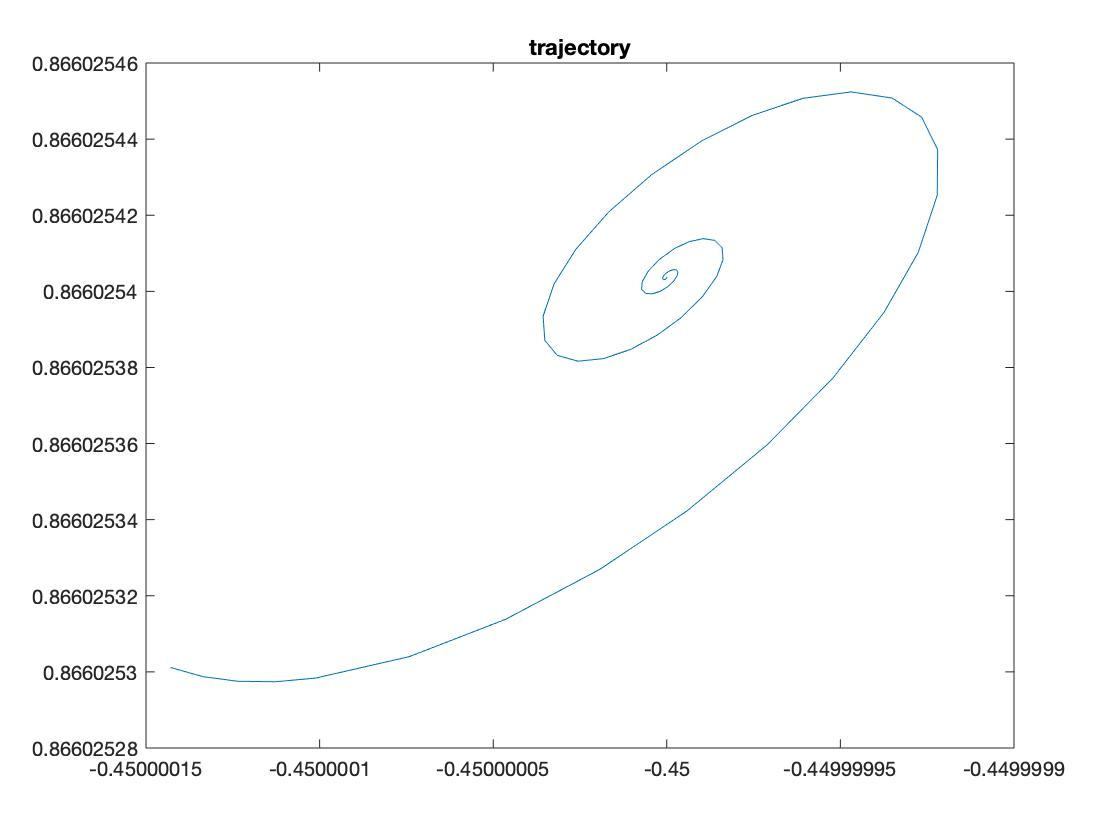
\includegraphics[width = 12cm, height = 8cm]{Q5(27).jpg}
\end{figure}
\newpage

Calculate the second derivatives of $\Omega$ at equilateral Lagrange points, we have the following: $$\Omega_{xx} = -\frac{3}{4}$$
$$\Omega_{xy} = \Omega_{yx} = \pm \frac{3\sqrt{3}}{2}(\frac{1}{2}-\mu)$$
$$\Omega_{yy} = -\frac{9}{4}$$
To investigate the stability of the Lagrange points, we perturb $\xi$ and $\eta$ in the x and y directions separately. Then we have the matrix: 

\[
\begin{pmatrix}
\dot {\xi} \\
\dot {\eta} \\
\ddot{\xi} \\
\ddot{\eta} \\
\end{pmatrix} 
=
\begin{pmatrix}
0 & 0 & 1 & 0\\
0 & 0 & 0 & 1\\
\Omega_{xx} & \Omega_{xy} & 0 & 2\\
\Omega_{xy} & \Omega_{yy}  & -2 & 0\\
\end{pmatrix}
\]

So we can see the matrix has 0 trace, and the sum of eigenvalues is 0. 
Calculate the characteristic equation : $x^4+x^2+\frac{27}{4}\mu(1-\mu)$.
The eigenvalues come in conjugate pairs, and since their sum is 0, the real parts of eigenvalues sum to 0, and therefore one must be positive if the other is negative. In order to have stability, we do not want a positive real part which leads to exponential growth, so all roots must be purely imaginary.
Then the quadratic equation $x^2+x+\frac{27}{4}\mu(1-\mu)$ must have two real negative roots, hence the determinant of it must be non-negative. No further restriction is needed as the sum of roots is -1, the product is $\frac{27}{4}\mu(1-\mu)>0$ as $mu \in \left(0,0.5\right]$.
Hence the critical value satisfies $$ 1-27\mu_{c} (1-\mu_{c}) = 0,\ \mu_{c} = 0.038521... $$
After executing numerical experimentation we can justify the result. For the stable cases, as we have two real eigenvalues, we are expected to have periodic motion, which is seen from some graphs of x,and y against t previously.
\section{Question 6}
The distribution of the Trojans are consistent with my findings above, as $\mu$ is below the critical value, both equilateral Lagrange points are stable. No analogue is observed in Earth-Moon system because the gravitational forces from the sun and other planets of the system are significant, while in the Solar-Jupiter system the distance is large and both are massive.
\newpage
\appendix
\section{Codes}
\subsection{Question 1}
\lstinputlisting{Dynsyst.m}
\lstinputlisting{Solver1.m}
\lstinputlisting{Check.m}
\subsection{Question 2}
\lstinputlisting{ModDynsyst.m}
\lstinputlisting{Modsolver.m}
\lstinputlisting{Question2.m}
\subsection{Question 3}
\lstinputlisting{Const.m}
\lstinputlisting{Potent.m}
\lstinputlisting{Fob_Reg.m}
\lstinputlisting{Question3.m}
\subsection{Question 4}
\lstinputlisting{Contour.m}
\lstinputlisting{LaPt.m}
\lstinputlisting{Question4.m}
\lstinputlisting{Question4_2.m}
\subsection{Question 5}
\lstinputlisting{Equi.m}
\lstinputlisting{Question5.m}
\end{document}